% Autor: Leonhard Segger, Alexander Neuwirth
% Datum: 2017-10-30
\documentclass[
	% Papierformat
	a4paper,
	% Schriftgröße (beliebige Größen mit „fontsize=Xpt“)
	12pt,
	% Schreibt die Papiergröße korrekt ins Ausgabedokument
	pagesize,
	% Sprache für z.B. Babel
	ngerman
]{scrartcl}

% Achtung: Die Reihenfolge der Pakete kann (leider) wichtig sein!
% Insbesondere sollten (so wie hier) babel, fontenc und inputenc (in dieser
% Reihenfolge) als Erstes und hyperref und cleveref (Reihenfolge auch hier
% beachten) als Letztes geladen werden!

% Silbentrennung etc.; Sprache wird durch Option bei \documentclass festgelegt
\usepackage{babel}
% Verwendung der Zeichentabelle T1 (Sonderzeichen etc.)
\usepackage[T1]{fontenc}
% Legt die Zeichenkodierung der Eingabedatei fest, z.B. UTF-8
\usepackage[utf8]{inputenc}
% Schriftart
\usepackage{lmodern}
% Zusätzliche Sonderzeichen
\usepackage{textcomp}

% Mathepaket (intlimits: Grenzen über/unter Integralzeichen)
\usepackage[intlimits]{amsmath}
% Ermöglicht die Nutzung von \SI{Zahl}{Einheit} u.a.
\usepackage{siunitx}
% Zum flexiblen Einbinden von Grafiken (\includegraphics)
\usepackage{graphicx}
% Abbildungen im Fließtext
\usepackage{wrapfig}
% Abbildungen nebeneinander (subfigure, subtable)
\usepackage{subcaption}
% Funktionen für Anführungszeichen
\usepackage{csquotes}
% Zitieren, Bibliographie
\usepackage{biblatex}


% Zur Darstellung von Webadressen
\usepackage{url}
%chemische Formeln
\usepackage[version=4]{mhchem}
% siunitx: Deutsche Ausgabe, Messfehler getrennt mit ± ausgeben
\usepackage{floatrow}
\floatsetup[table]{capposition=top}
% Verlinkt Textstellen im PDF-Dokument
\usepackage[unicode]{hyperref}
% "Schlaue" Referenzen (nach hyperref laden!)
\usepackage{cleveref}
\sisetup{
	locale=DE,
	separate-uncertainty
}
%\bibliography{6Mi_M3_29-11-2017_References}

\begin{document}
	
	\begin{titlepage}
		\centering
		{\scshape\LARGE Versuchsbericht zu \par}
		\vspace{1cm}
		{\scshape\huge E1 - Gleich- und Wechselstrom\par}
		\vspace{2.5cm}
		{\LARGE Gruppe 6Mi \par}
		\vspace{0.5cm}
		
		{\large Alexander Neuwirth (E-Mail: a\_neuw01@wwu.de) \par}
		{\large Leonhard Segger (E-Mail: l\_segg03@uni-muenster.de) \par}
		\vfill
		
		durchgeführt am 20.12.2017\par 
		betreut von\par
		{\large Philipp Eickholt}            
		
		\vfill
		
		{\large \today\par}
	\end{titlepage}
	\tableofcontents
	\newpage


	\section{Kurzfassung}
	%TODO Hypothese	und deren Ergebnis
	%TODO Ergebnisse, auch Zahlen, mindestens wenn's halbwegs Sinn ergibt
	%TODO Was wurde gemacht
	Es wurden zwei Experimente zu Gleich- und Wechselstrom bzw. dem Innenwiderstand von Stromquellen durchgeführt.
	Im ersten Experiment wurde durch Messung der Klemmspannung in Abhängigkeit vom Außenwiderstand in einem einfachen Stromkreis der Innenwiderstand von Akkumulatorzellen untersucht.
	Da hier der Innenwiderstand durch einen angelöteten Widerstand künstlich erhöht war, war zu erwarten, dass der berechnete Gesamtinnenwiderstand sich nur geringfügig (nämlich um den tatsächlichen Innenwiderstand der Zelle) von dem auf dem Widerstand angegebenen Widerstand unterscheidet.
	Dies konnte experimentell nicht bestätigt werden, was entweder auf einen Fehler dieser Annahme oder einen Fehler bei der Messung schließen lässt.
	\par 
	Im zweiten Experiment wurde die Leistungsaufnahme verschiedener Verbraucher in Abhängigkeit von der Größe und Form (Gleich- oder Wechselspannung) der angelegten Spannung untersucht.
	Zunächst wurde hier die Leistungsaufnahme eines ohmschen Widerstandes gemessen, wobei die grobe Schätzung des Widerstandes anhand der Stellung des Potentiometers bestätigt werden konnte.
	Nicht bestätigt werden konnte jedoch der Zusammenhang zwischen Spannung, Stromstärke und Leistung.
	Auch wurde Wirkwiderstand, Innenwiderstand und Phasenwinkel einer Spule sowie Betrag und Phase des Wechselstromwiderstandes der Kombination von Spule und Kondensator bestimmt.
	Hierbei war zu erwarten, dass die Messungen ähnliche Werte für Widerstand und Kapazität ergeben, wie auf Widerstand und Kondensator angegeben war.
	Dies konnte tatsächlich anhand der Messwerte in beiden Fällen bestätigt werden.
	Auch konnte gezeigt werden, dass der theoretisch erwartete Zusammenhang zwischen Impedanz und Wirkwiderstand bei Wechselstrombetrieb und Innenwiderstand bei Gleichstrombetrieb besteht.
	
	\section{Methoden}
	%TODO Bilder von der Website klauen
	Zunächst wurde ein einfacher Stromkreis aufgebaut, mit dem der Innenwiderstand von Akkumulatorzellen gemessen werden konnte.
	Dieser bestand aus einem veränderlichen Lastwiderstand, der Stromquelle und einem Spannungsmessgerät, mit dem die Klemmspannung der Stromquelle erfasst wurde.
	Dann wurde der Lastwiderstand verändert und die Klemmspannung über der Stromquelle gemessen.
	Dies wurde drei mal mit verschiedenen Stromquellen durchgeführt.
	Hier wurde zunächst eine einzelne Akkumulatorzelle, dann drei Zellen parallel und zuletzt drei Zellen in Reihenschaltung verwendet.
	Dabei hatten die Zellen einen künstlich (durch einen eingebauten Widerstand) erhöhten Innenwiderstand.
	Dieser Widerstand wurde abgelesen.
	\par
	
	\begin{figure}[tb]
		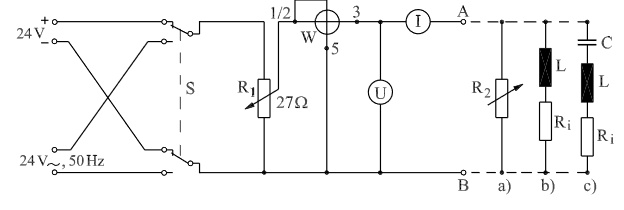
\includegraphics[width=0.8\textwidth]{Schaltkreis2}
		\centering
		\caption{Der Schaltkreis, der zur Messung der Leistungsaufnahme verschiedener Verbraucher benutzt wurde.}
		\label{SK2}
		\centering
	\end{figure}
	
	Dann wurde die in \cref{SK2} dargestellte Schaltung zur Messung der Leistungsaufnahme verschiedener Verbraucher bei Gleich- und Wechselstrom aufgebaut.
	Hierfür wurde zunächst für zwei verschiedene Voltmeter deren Verlustleistung in Abhängigkeit von Gleich- bzw. Wechselspannung beobachtet, indem die Schaltung in \cref{SK2} ohne Verbraucher verwendet wurde, um einer Entscheidung treffen zu können, welches Messgerät im Folgenden verwendet werden sollte und inwiefern dessen Verlustleistung berücksichtigt werden muss.
	Dann wurde für ein festes $ R_2 $ bei Gleich- und Wechselstrom Spannung, Stromstärke und Leistung für fünf verschiedene Widerstände $ R_1 $ bei gemessen.
	Hierbei wurde das Potentiometer mit dem Widerstand $ R_2 $ so eingestellt, dass ein möglichst großer Messbereich der Messgeräte genutzt werden konnte.
	Dann wurde diese Messung für eine Spule sowie eine Spule mit Kondensator wiederholt. 
	
	\section{Ergebnisse und Diskussion}
	\subsection{Beobachtung}
	Es wird davon ausgegangen, dass die Unsicherheiten der Messapparaturen im Vergleich zu den Ableseungenauigkeiten verschwinden (\cref{Tabelle_Unsicherheiten}).
	Die Fortpflanzung der Fehler wurde immer gemäß \cref{Partielle_Unsicherheiten} berechnet.
	\begin{equation}
		u(y) = \sqrt{  \sum_{i=0}^{N} \left( \frac{\partial f}{\partial x_i}u(x_i)\right)^2  }
		\label{Partielle_Unsicherheiten}
	\end{equation}
	\begin{table}[tb]
		\centering
		\begin{tabular}{ r | c | c | c}
			& Voltmeter & Amperemeter & Wattmeter \\ \hline 
			 Messunsicherheit& \SI{0,0204}{V}&  \SI{0,004}{A}&  \SI{0,04}{W}\\

		\end{tabular}
		\caption{Unsicherheiten verschiedener Messapparaturen.}
		\label{Tabelle_Unsicherheiten} 
	\end{table}
	
	\subsubsection{Innenwiderstand}
	In \cref{Spannung1} ist die Klemmspannung gegen den Strom, der sich aus $I = U/R$ ergeben hat, aufgetragen. 
	Es wurde ein linearer Fit durchgeführt, da nach der Theorie ein linearer Zusammenhang besteht. 
	Die Steigung der Geraden ist der (negative) Innenwiderstand $R_\text{i} = \SI{27,19 \pm 0,47}{\Omega}$.

	Trägt man die Leistung gegen den Außenwiderstand auf, ist zu erwarten, dass (genau) ein Maximum bei $R_\text{i}  R_\text{a}$ liegt. %TODO maybe lieber mit cdot. sieht seltsam aus
	\cref{Leistung1} stellt dies und einen Fit mit dem \enquote{Scaled Levenberg-Marquardt}-Algorithmus, welcher die Methode der kleinsten Quadrate verwendet, dar. 
	Die für den Fit verwendete Funktion ist:
	\begin{equation}
		f(x)=a\frac{x}{(x+b)^2}
	\end{equation}
	Es ergibt sich ein Parameter $b = \SI{29,51}{}$ ohne Unsicherheit, deshalb haben wir diese als relative Unsicherheit mit 2\% abgeschätzt. %Wird er nicht mögen
	Folglich ist $R_\text{i} = \SI{29,51 \pm 0,59}{\Omega}$.

	Analog kann man aus \crefrange{Spannung3Reihe}{Leistung3Parallel} die Innenwiderstände für drei parallel, bzw. in Reihe, geschaltete Akkus erhalten. 
	Der Widerstand des Voltmeters beim Bestimmen der Leerlaufspannung wurde auf \SI{2000}{\Omega} abgeschätzt.

	In \cref{Tabelle_Innenwiderstaende} sind die ermittelten Innenwiderstände aufgelistet. 
	Aus diesen Widerständen lassen sich die Innenwiderstände der einzelnen Akkus bestimmen.
	\cref{Tabelle_Innenwiderstaende2} zeigt diese. 


	\subsubsection*{Zusatzfrage}
	Eine Stromquelle soll einen möglichst konstanten Strom liefern. Das wird erreicht durch einen möglichst hohen Innenwiderstand, also eine Reihenschaltung der Spannungsquellen. Für eine Spannungsquelle bietet sich eine Parallelschaltung an, da der Innenwiderstand gering und somit die Spannung konstant gehalten werden kann.
	\begin{table}[tb]
		\centering
		\begin{tabular}{ r | c | c | c}
			Innenwiderstand& Ein Akku & 3 Akkus Reihe & 3 Akkus Parallel \\ \hline
			aus Klemmspannung& \SI{27,19 \pm 0,47 }{\Omega}& \SI{81,24 \pm 1,06 }{\Omega}&  \SI{9,73 \pm 0,20 }{\Omega} \\
			aus Leistung & \SI{29,51 \pm 0,59 }{\Omega}&  \SI{77,53 \pm 1,55 }{\Omega}&  \SI{9,79 \pm 0,19 }{\Omega}\\

		\end{tabular}
		\caption{Gemessener Innenwiderstand.}
		\label{Tabelle_Innenwiderstaende} 
	\end{table}
	\begin{table}[tb]
		\centering
		\begin{tabular}{ r | c | c | c}
			Innenwiderstand& Ein Akku & Akku Reihe & Akku Parallel \\ \hline
			aus Klemmspannung& \SI{27,19 \pm 0,47 }{\Omega}& \SI{27,08 \pm 0,35 }{\Omega}&  \SI{29,19 \pm 0,60 }{\Omega} \\
			aus Leistung & \SI{29,51 \pm 0,59 }{\Omega}&  \SI{25,84 \pm 0,52 }{\Omega}&  \SI{29,37 \pm 0,57 }{\Omega}\\

		\end{tabular}
		\caption{Berechneter Innenwiderstand von jeweils einem Akku.}
		\label{Tabelle_Innenwiderstaende2} 
	\end{table}

	\begin{figure}[tb]
		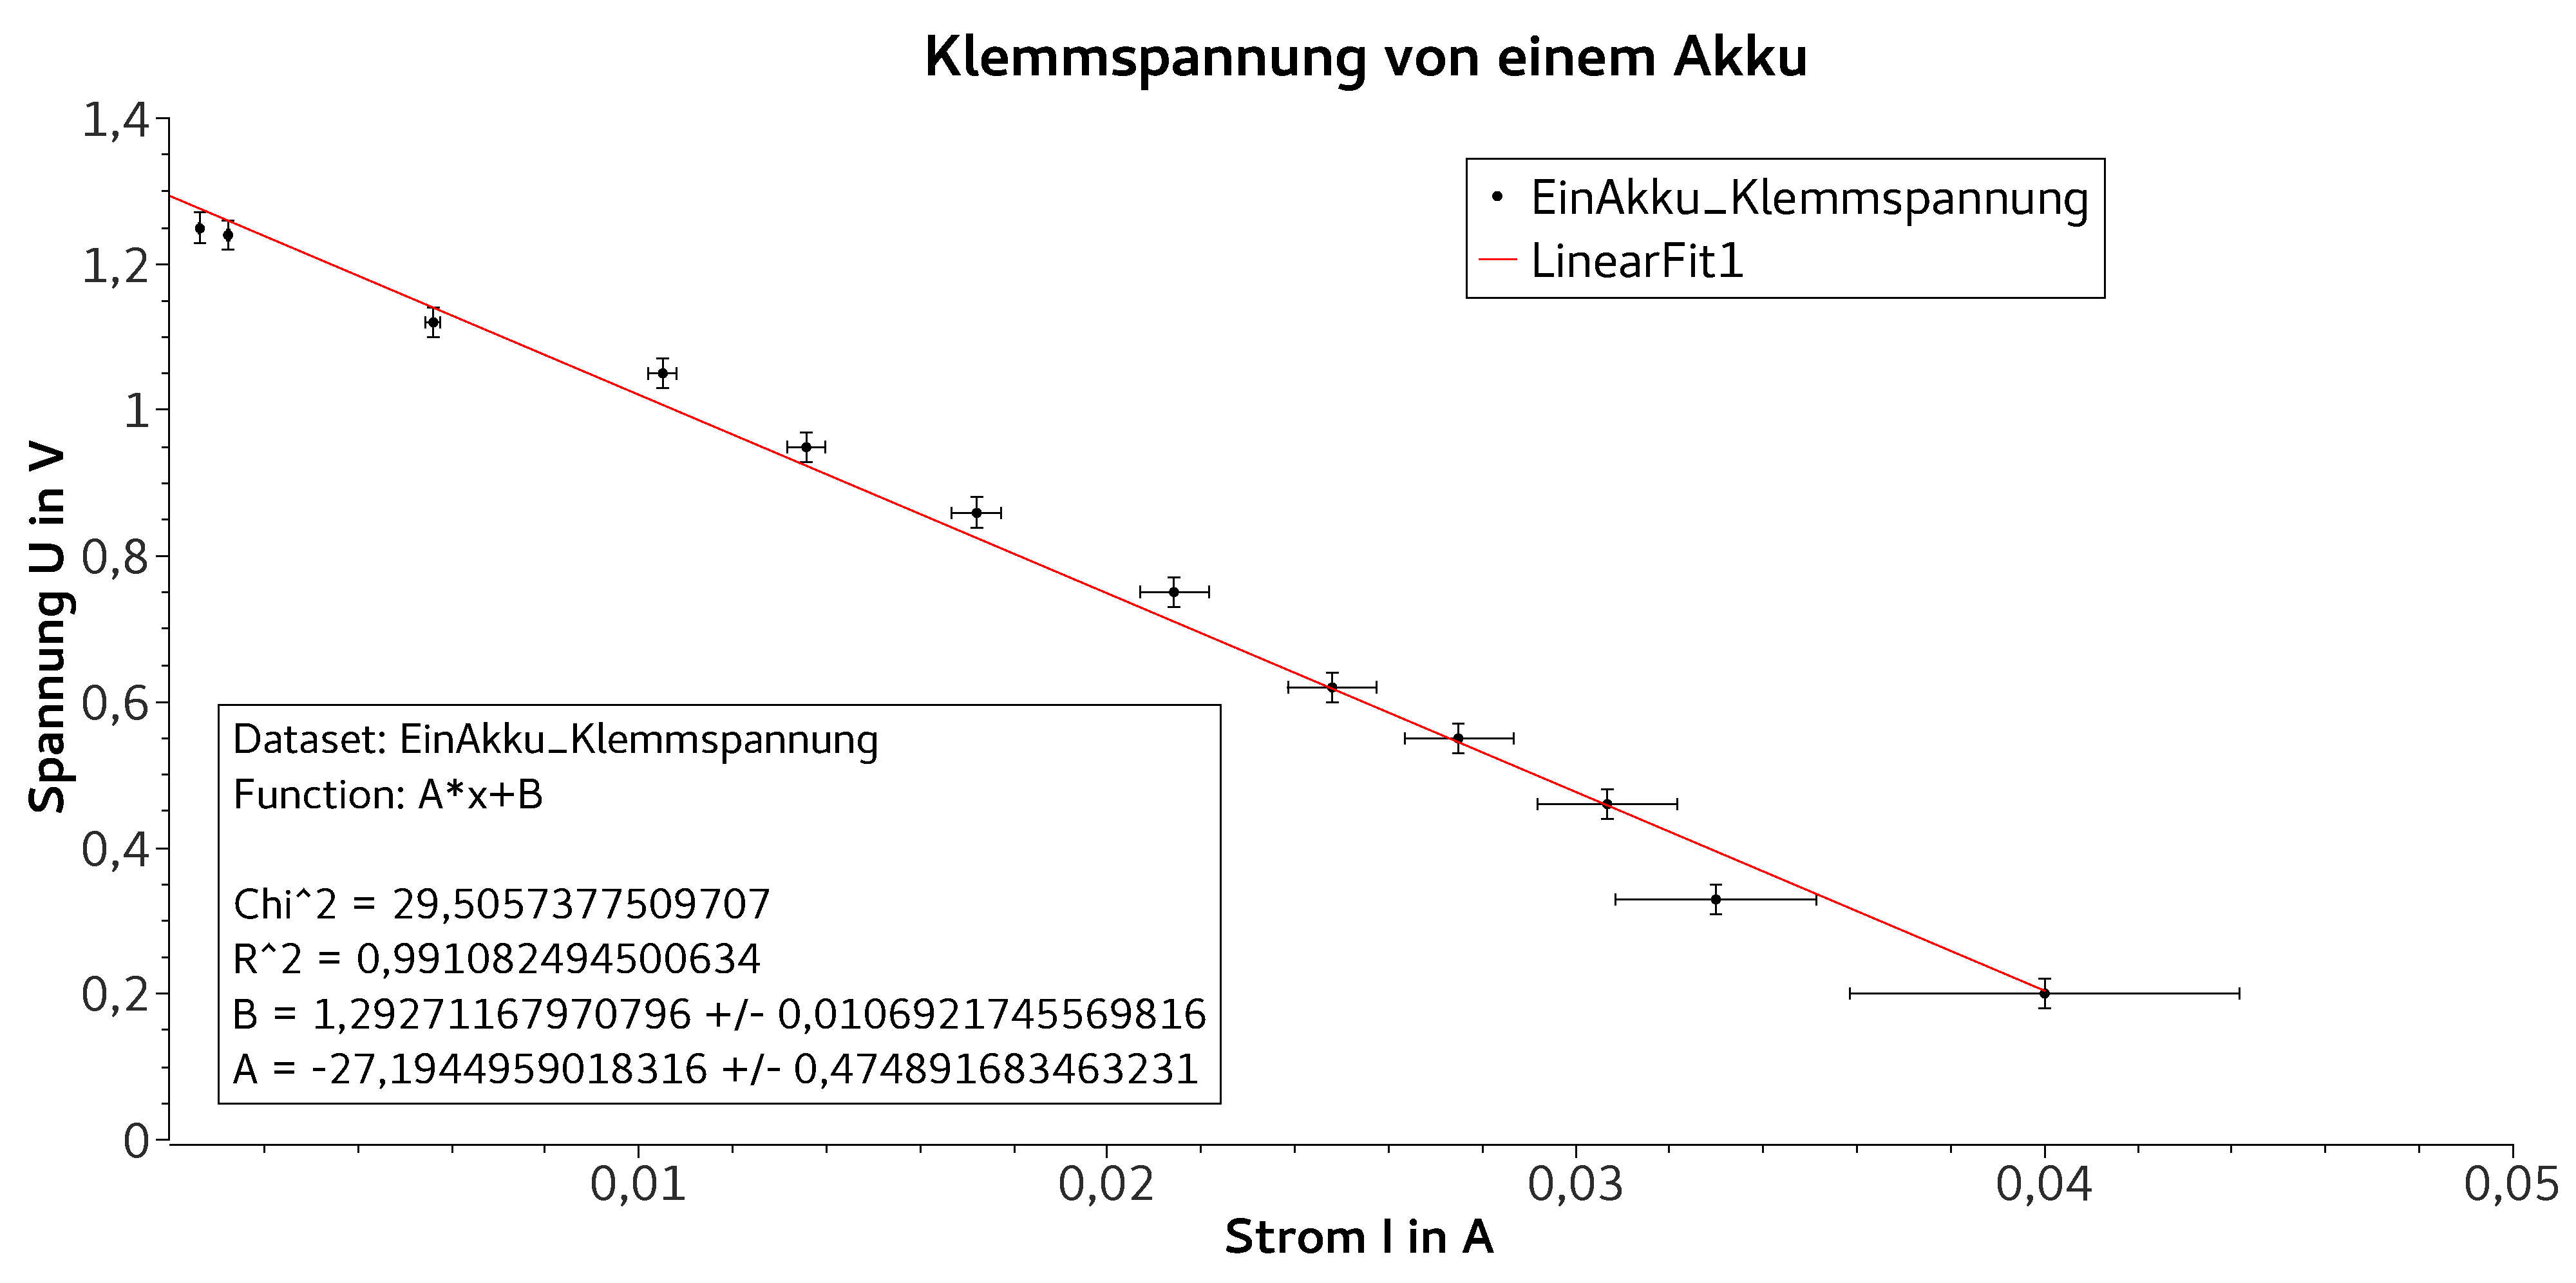
\includegraphics[width=1\textwidth]{Spannung1}
		\centering
		\caption{Die gemessene Klemmspannung bei einem Akku ist gegen den Strom aufgetragen.}
		\label{Spannung1}
		\centering
	\end{figure} 
	\begin{figure}[tb]
		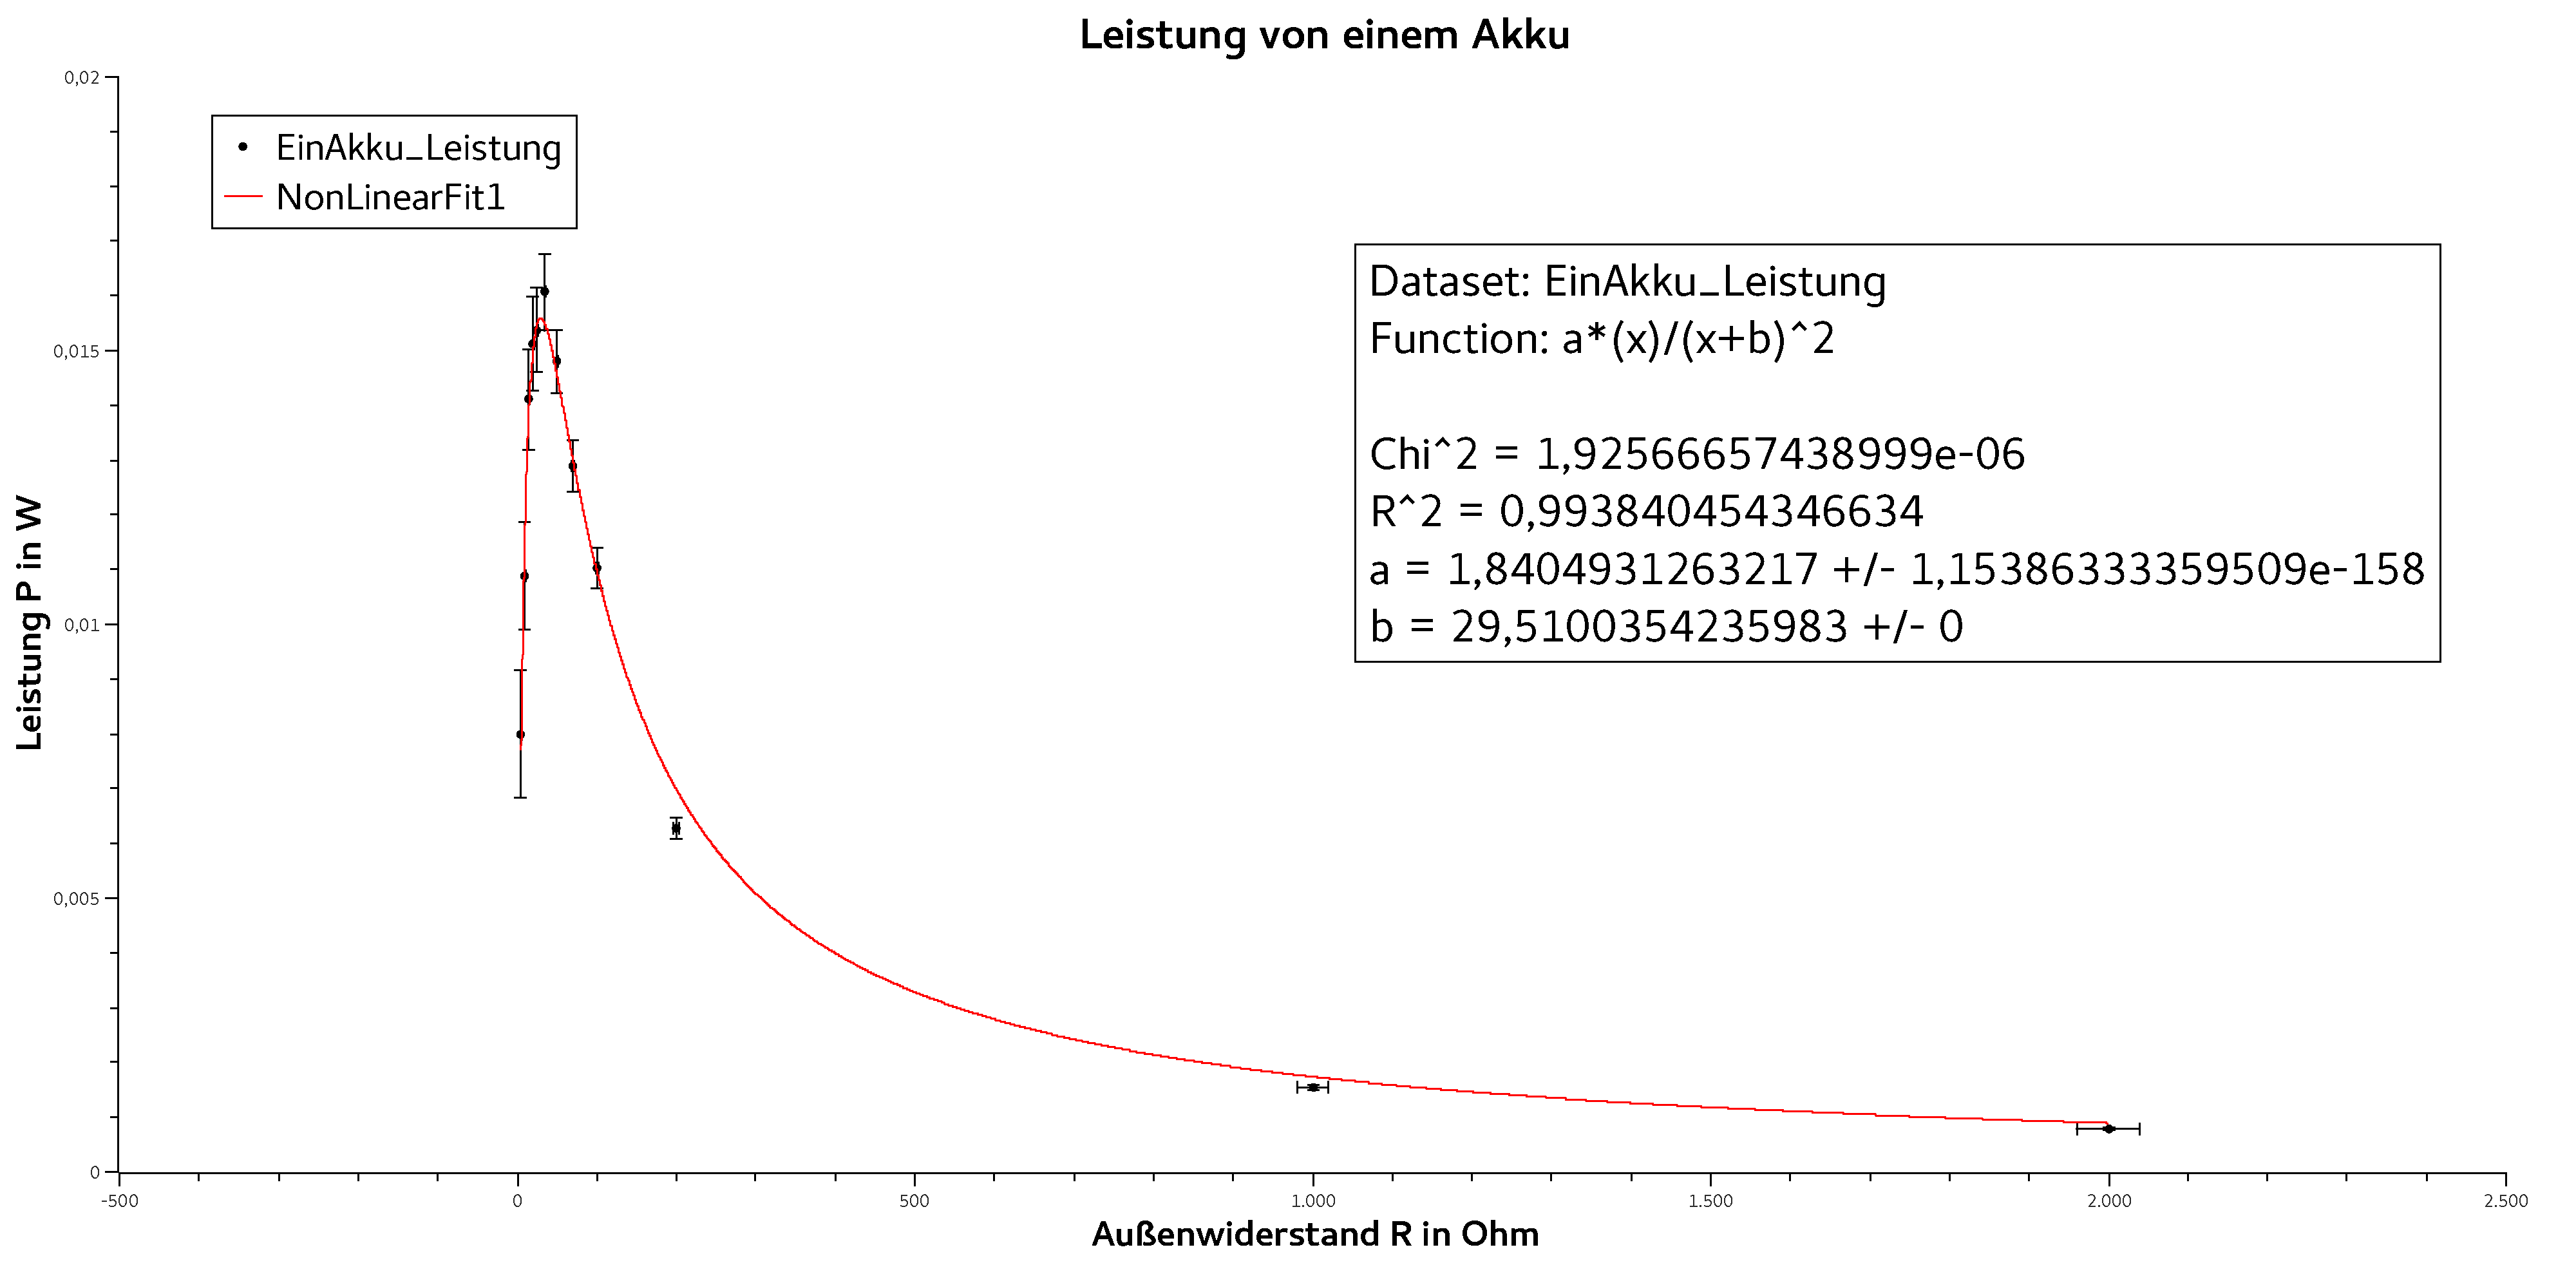
\includegraphics[width=1\textwidth]{Leistung1}
		\centering
		\caption{Die gemessene Leistung bei einem Akku ist gegen den Außenwiderstand aufgetragen.}
		\label{Leistung1}
		\centering
	\end{figure}
	\begin{figure}[tb]
		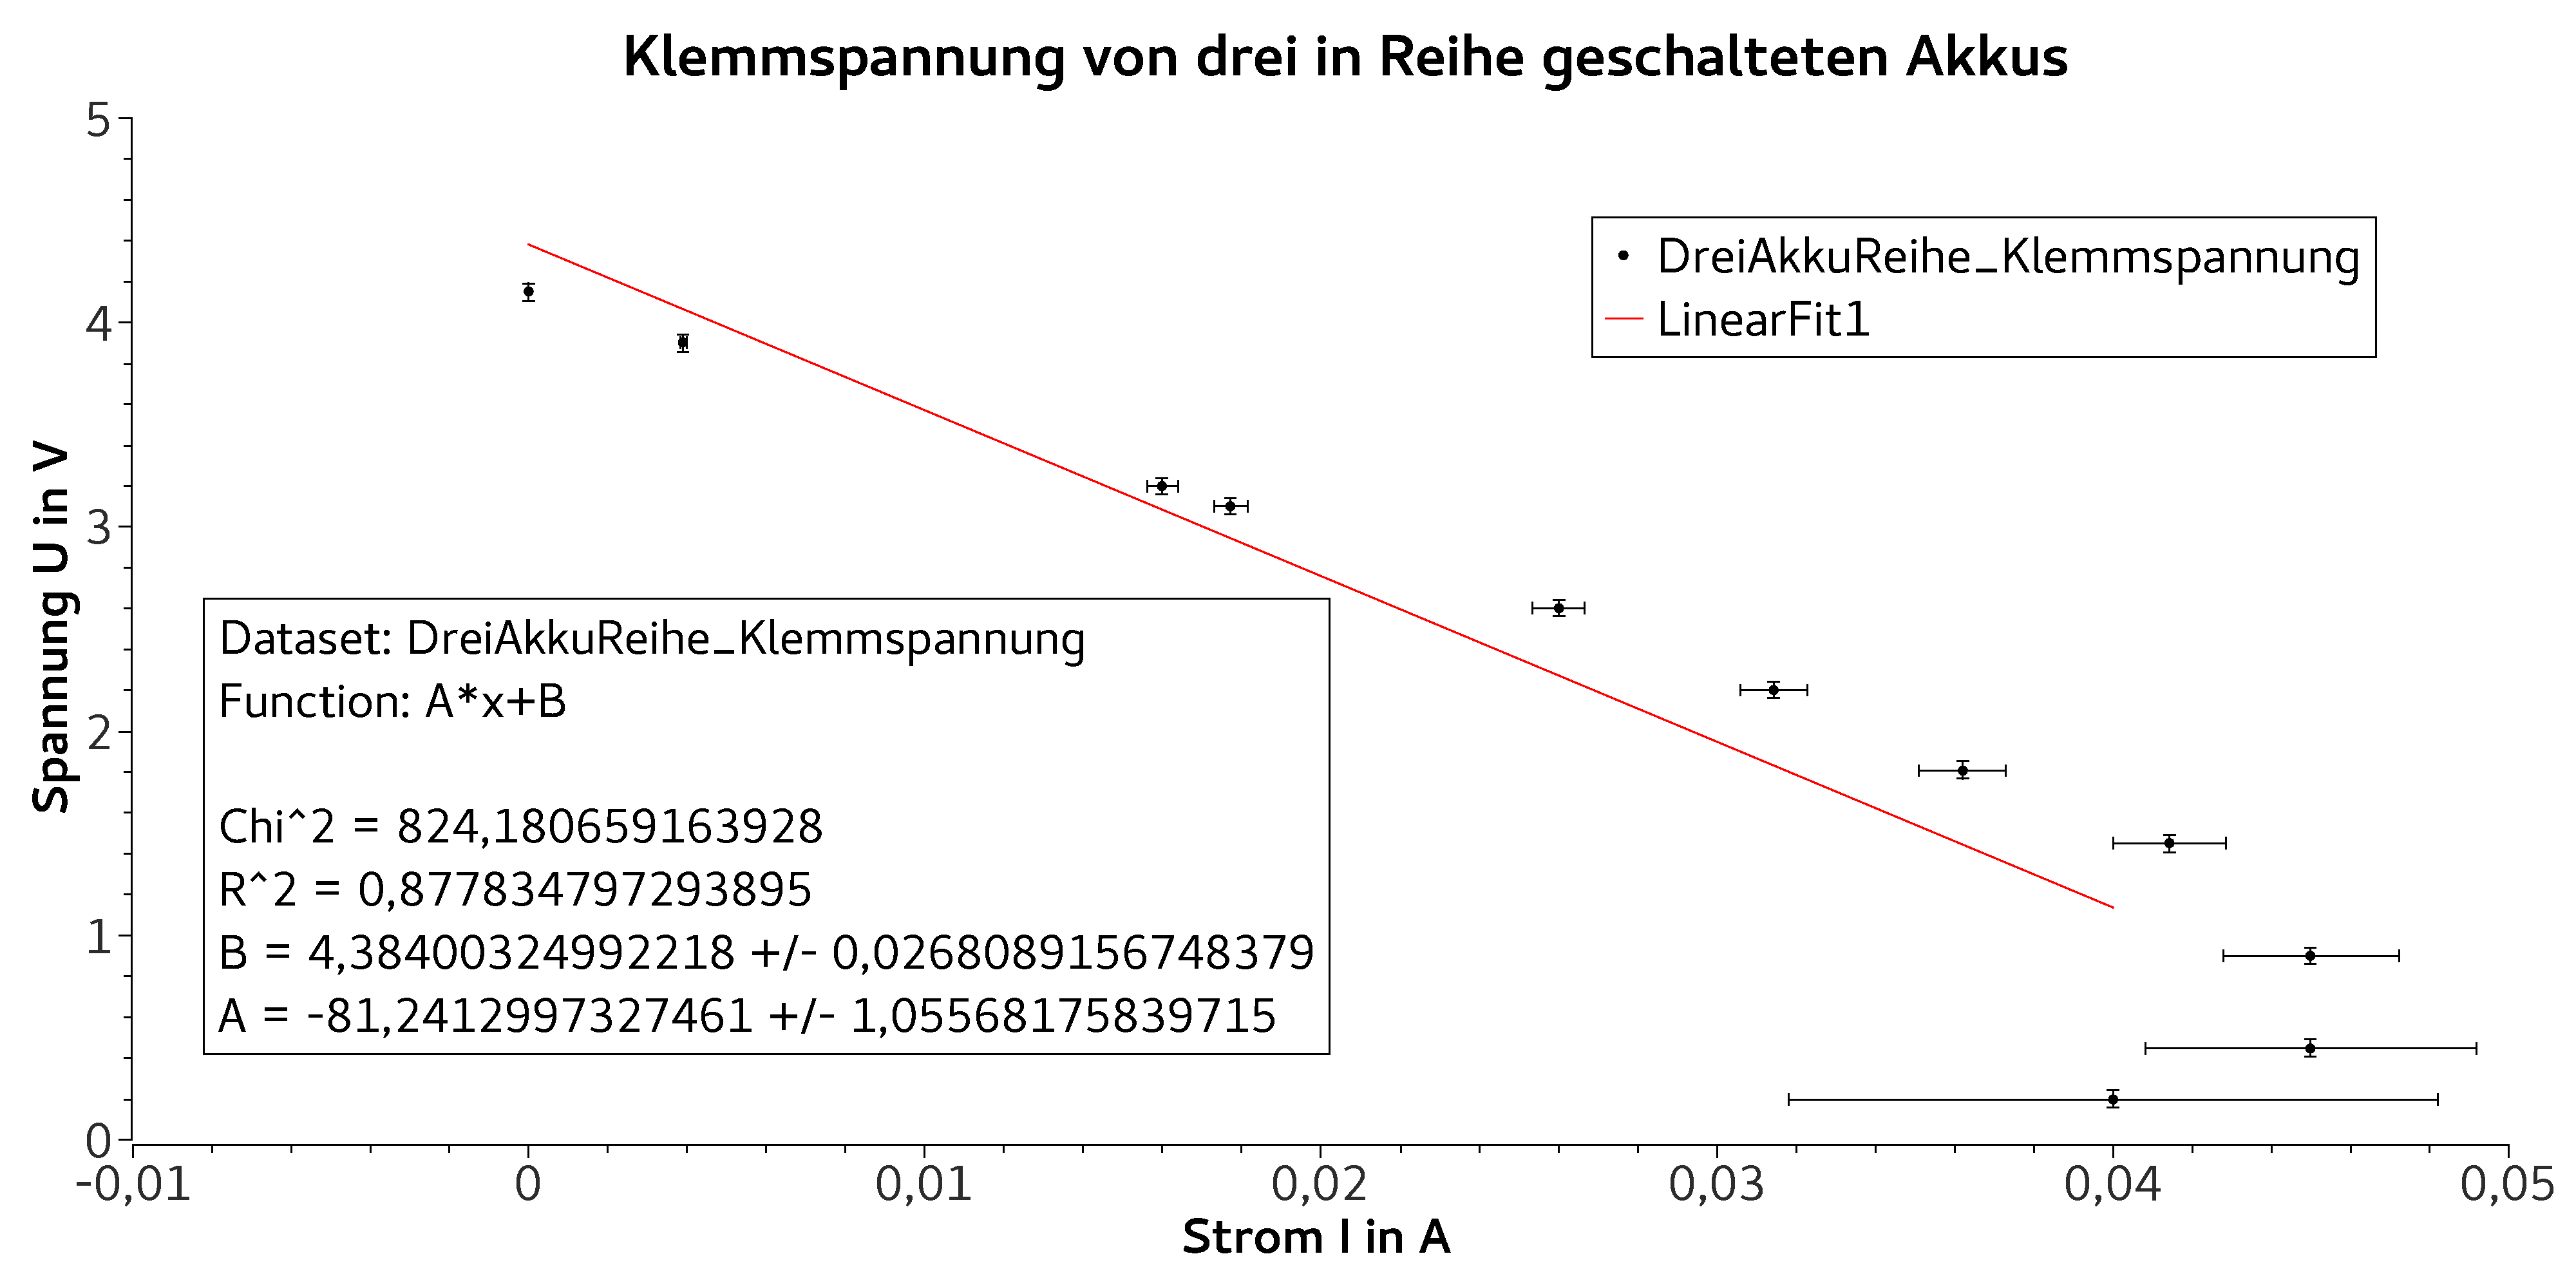
\includegraphics[width=1\textwidth]{Spannung3Reihe}
		\centering
		\caption{Die gemessene Klemmspannung bei drei in Reihe geschateten Akkus ist gegen den Strom aufgetragen. Es wurde mit der doppelten Ableseungenauigkeit gerechnet also \SI{0,0408}{V}}
		\label{Spannung3Reihe}
		\centering
	\end{figure} 
	\begin{figure}[tb]
		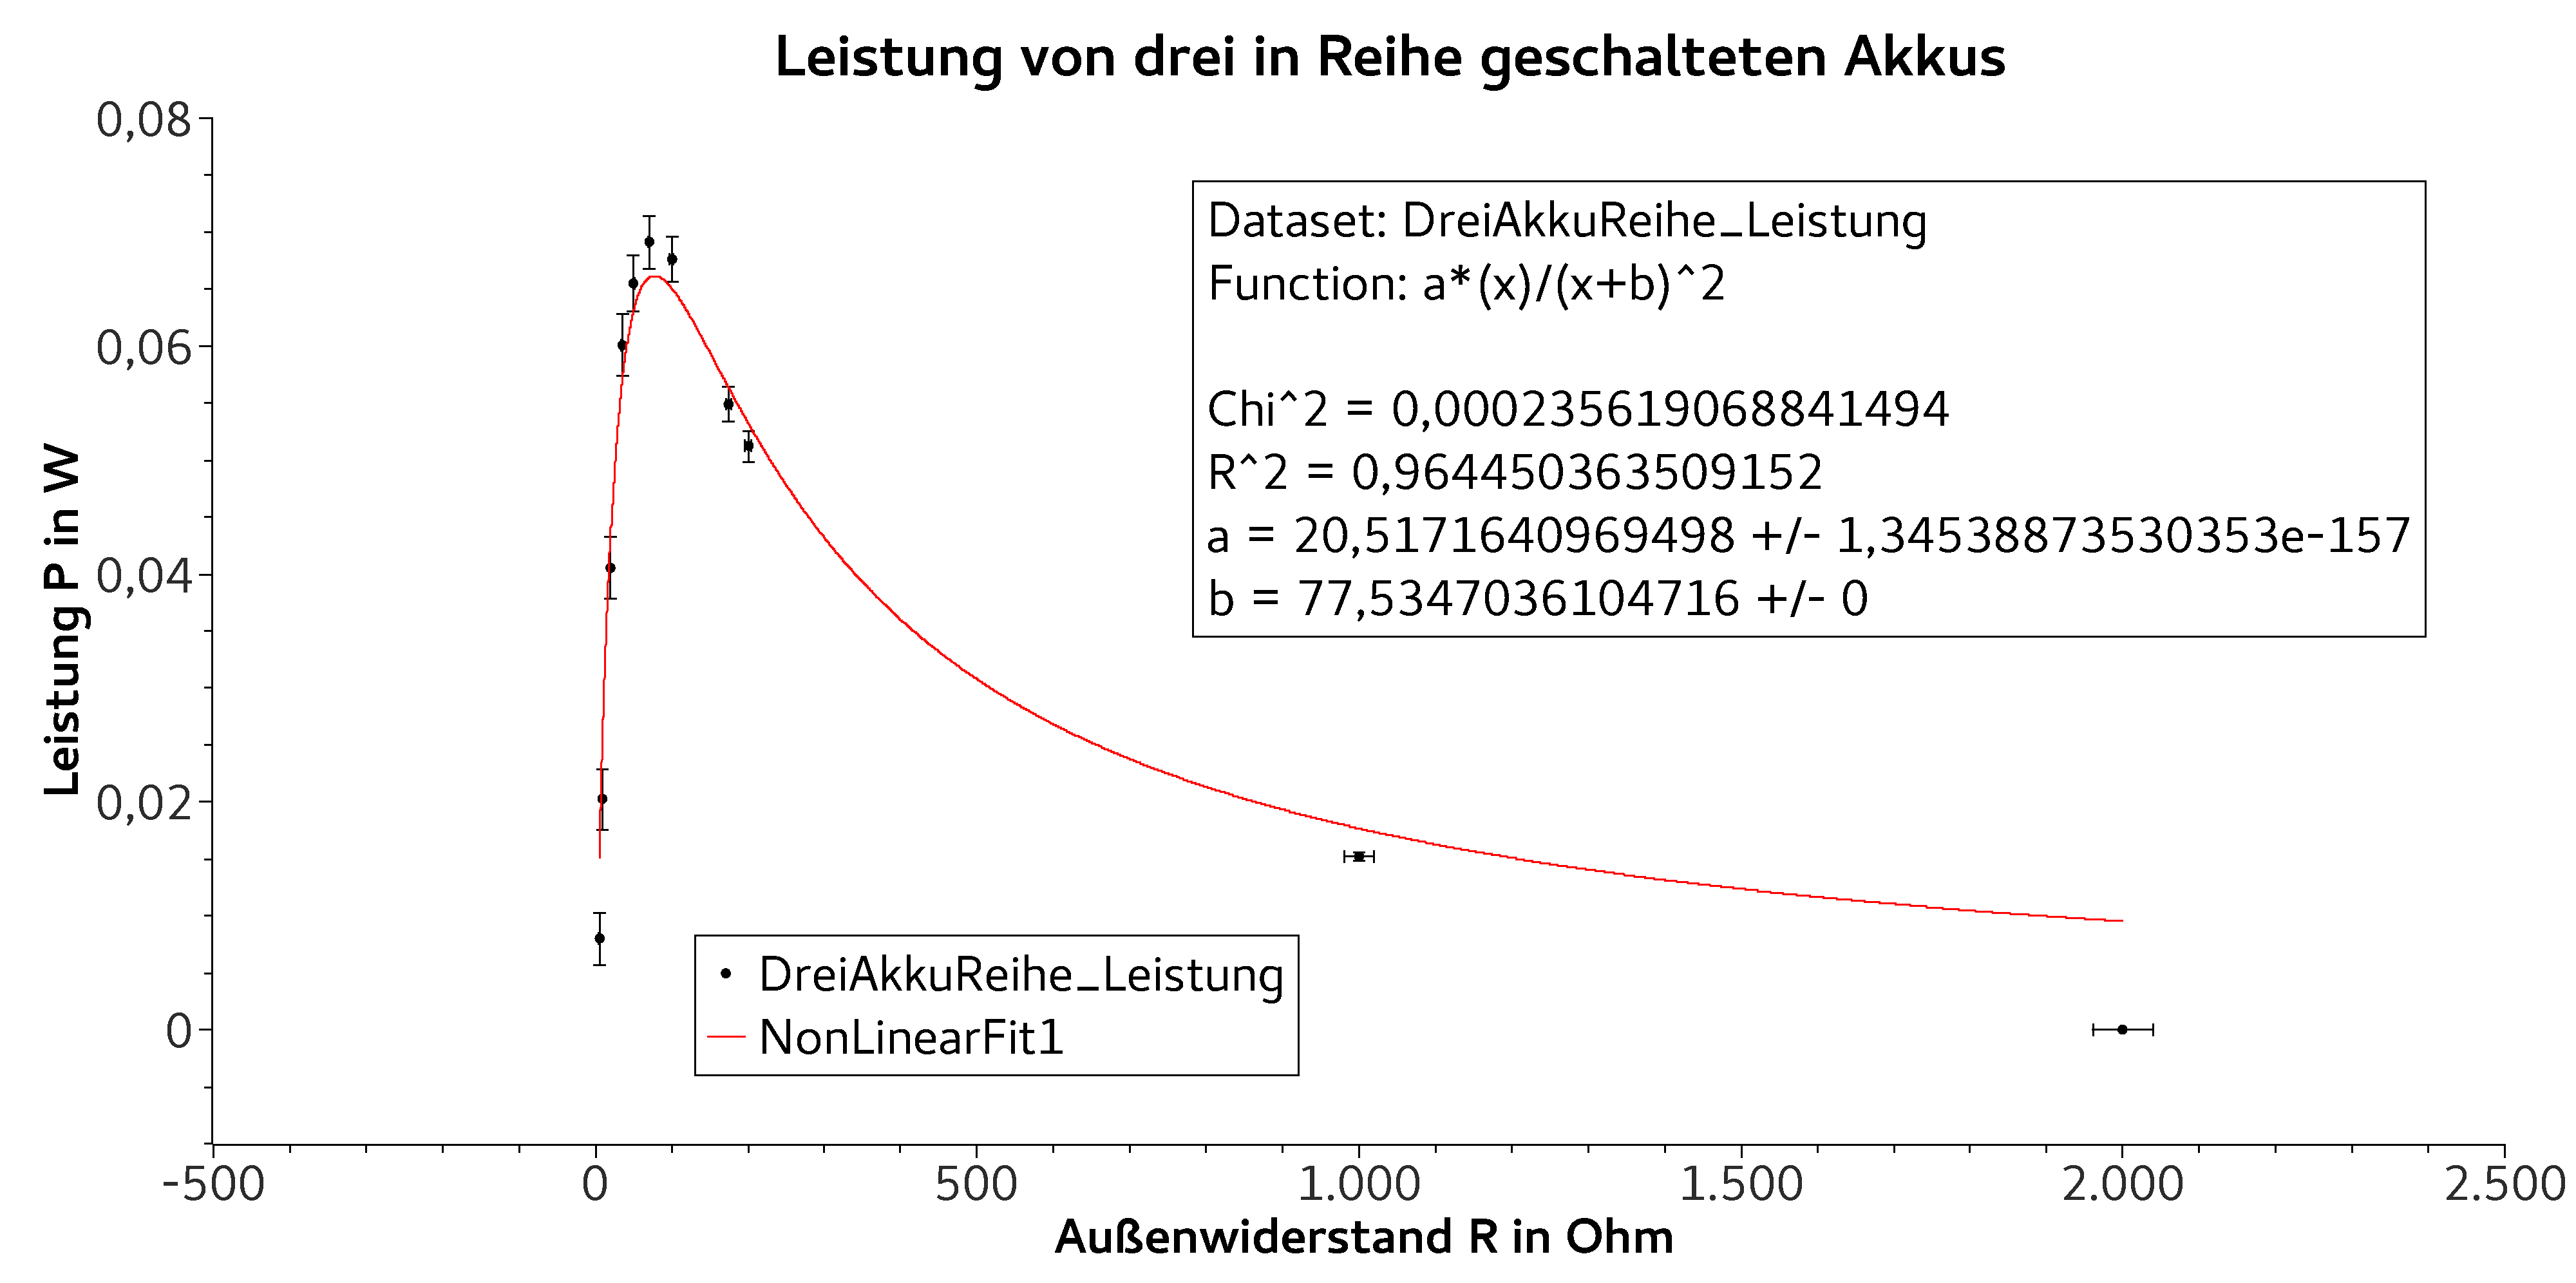
\includegraphics[width=1\textwidth]{Leistung3Reihe}
		\centering
		\caption{Die gemessene Leistung bei drei in Reie geschalteten Akkus ist gegen den Außenwiderstand aufgetragen. Es wurde mit der doppelten Ableseungenauigkeit gerechnet also \SI{0,0408}{V}}
		\label{Leistung3Reihe}
		\centering
	\end{figure}
	
	\begin{figure}[tb]
		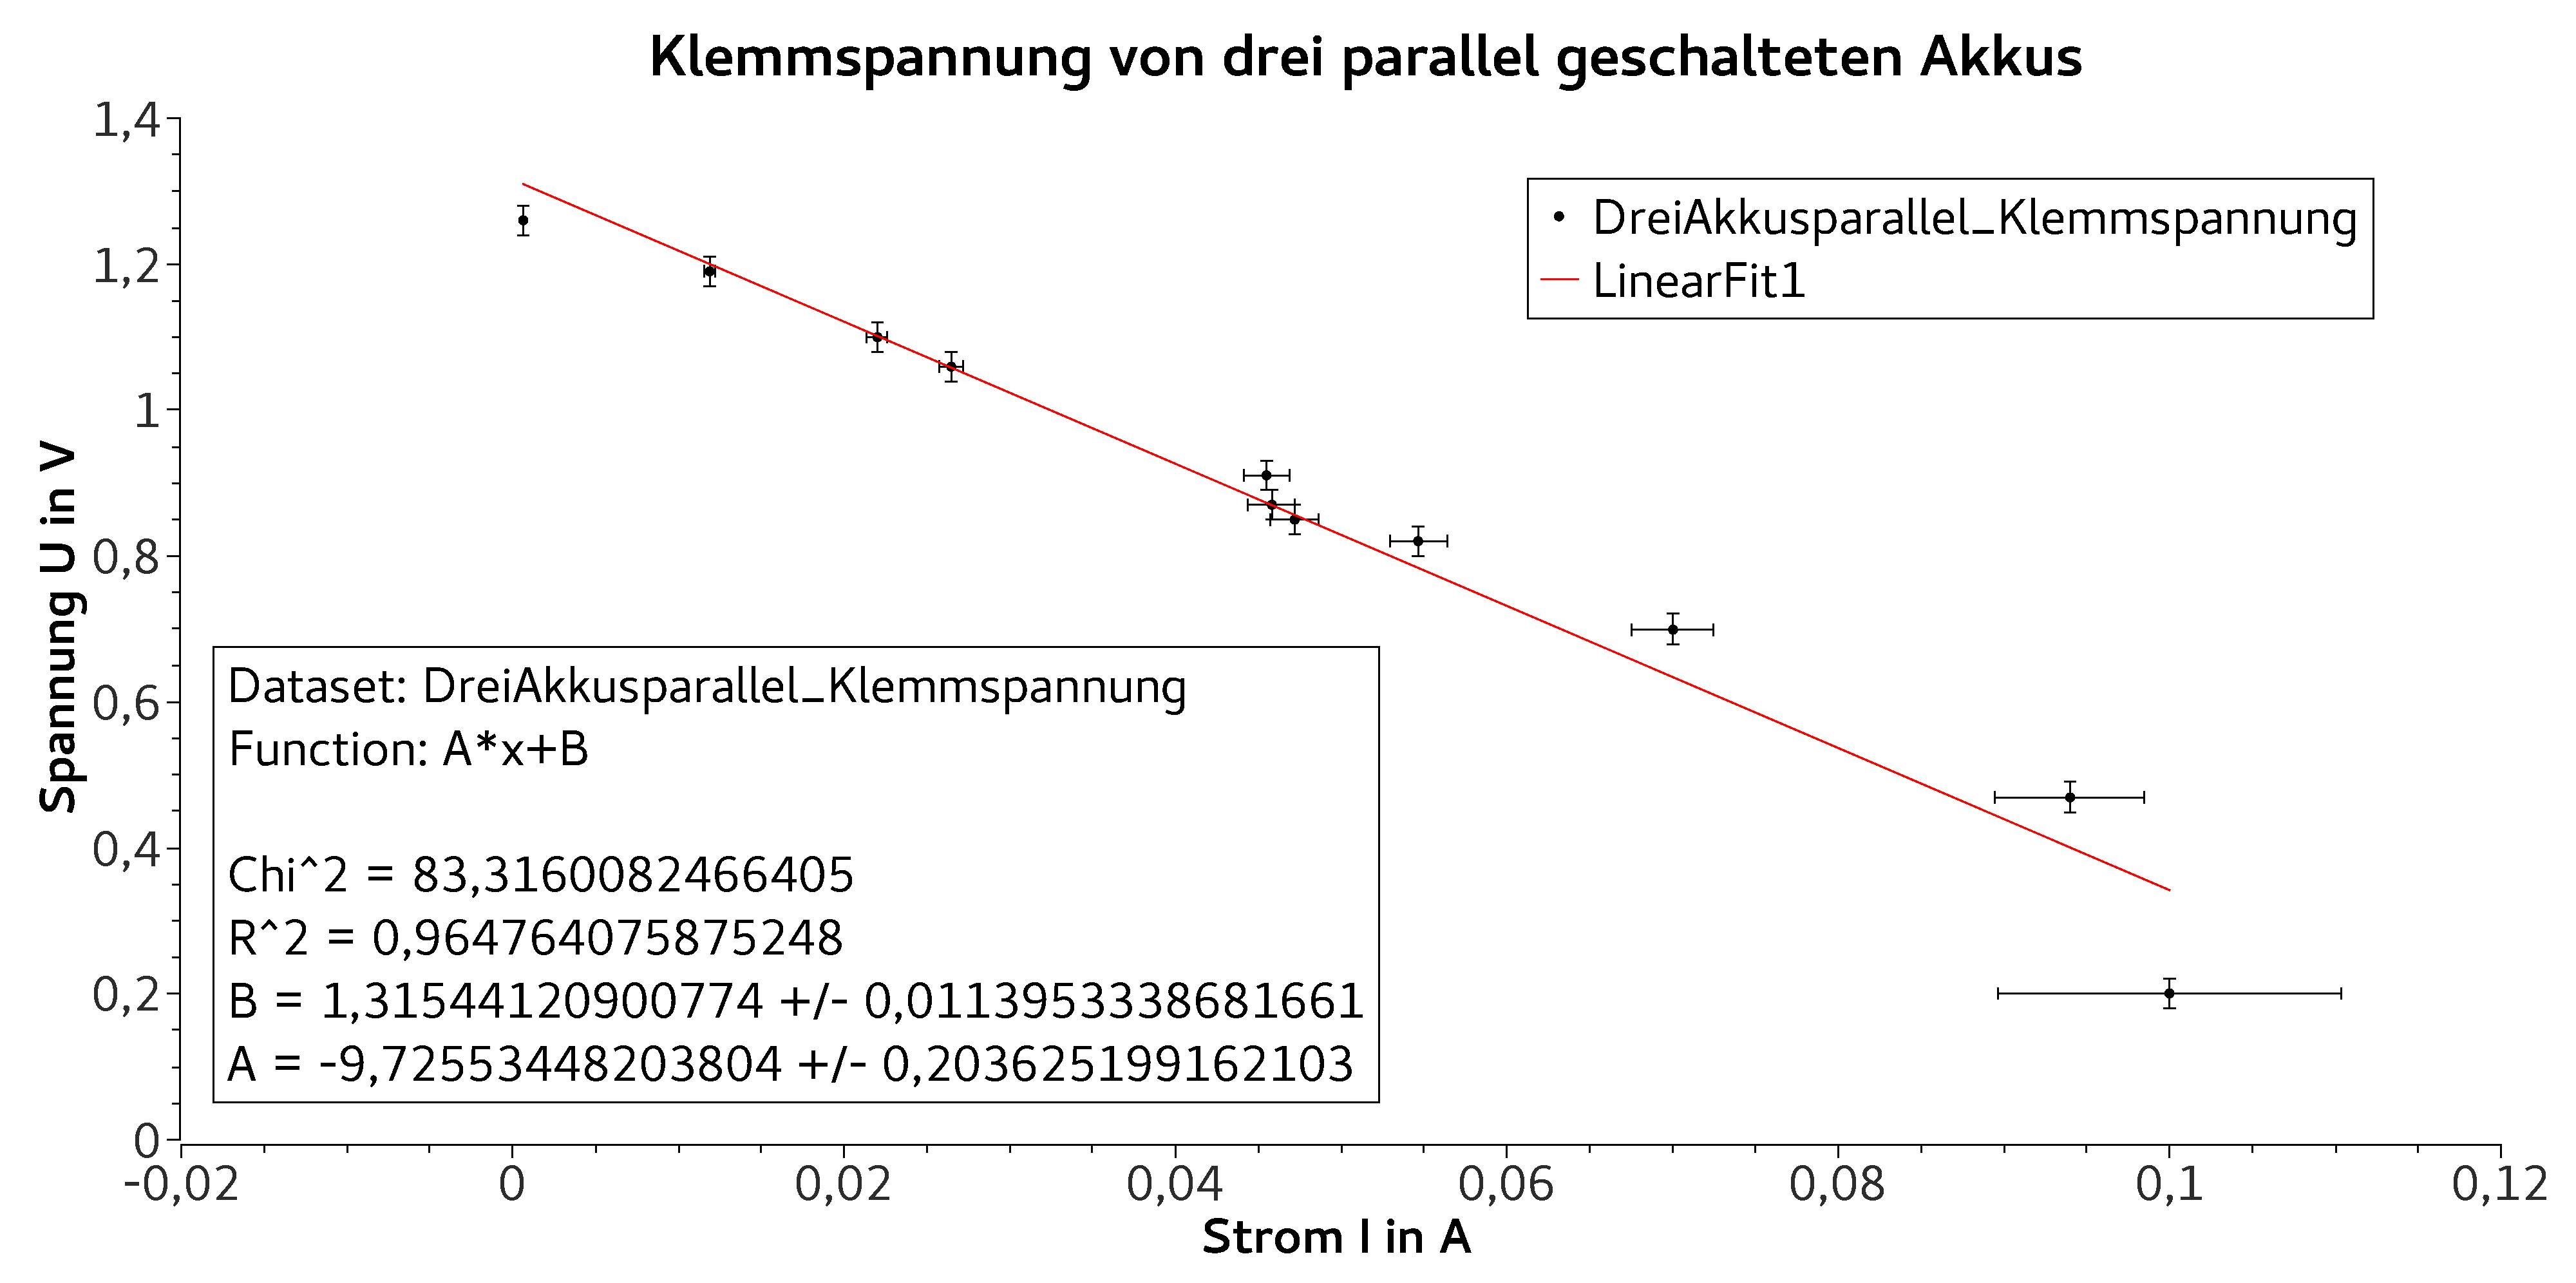
\includegraphics[width=1\textwidth]{Spannung3Parallel}
		\centering
		\caption{Die gemessene Klemmspannung bei 3 parallelen Akkus ist gegen den Strom aufgetragen.}
		\label{Spannung3Parallel}
		\centering
	\end{figure}

	\begin{figure}[tb]
		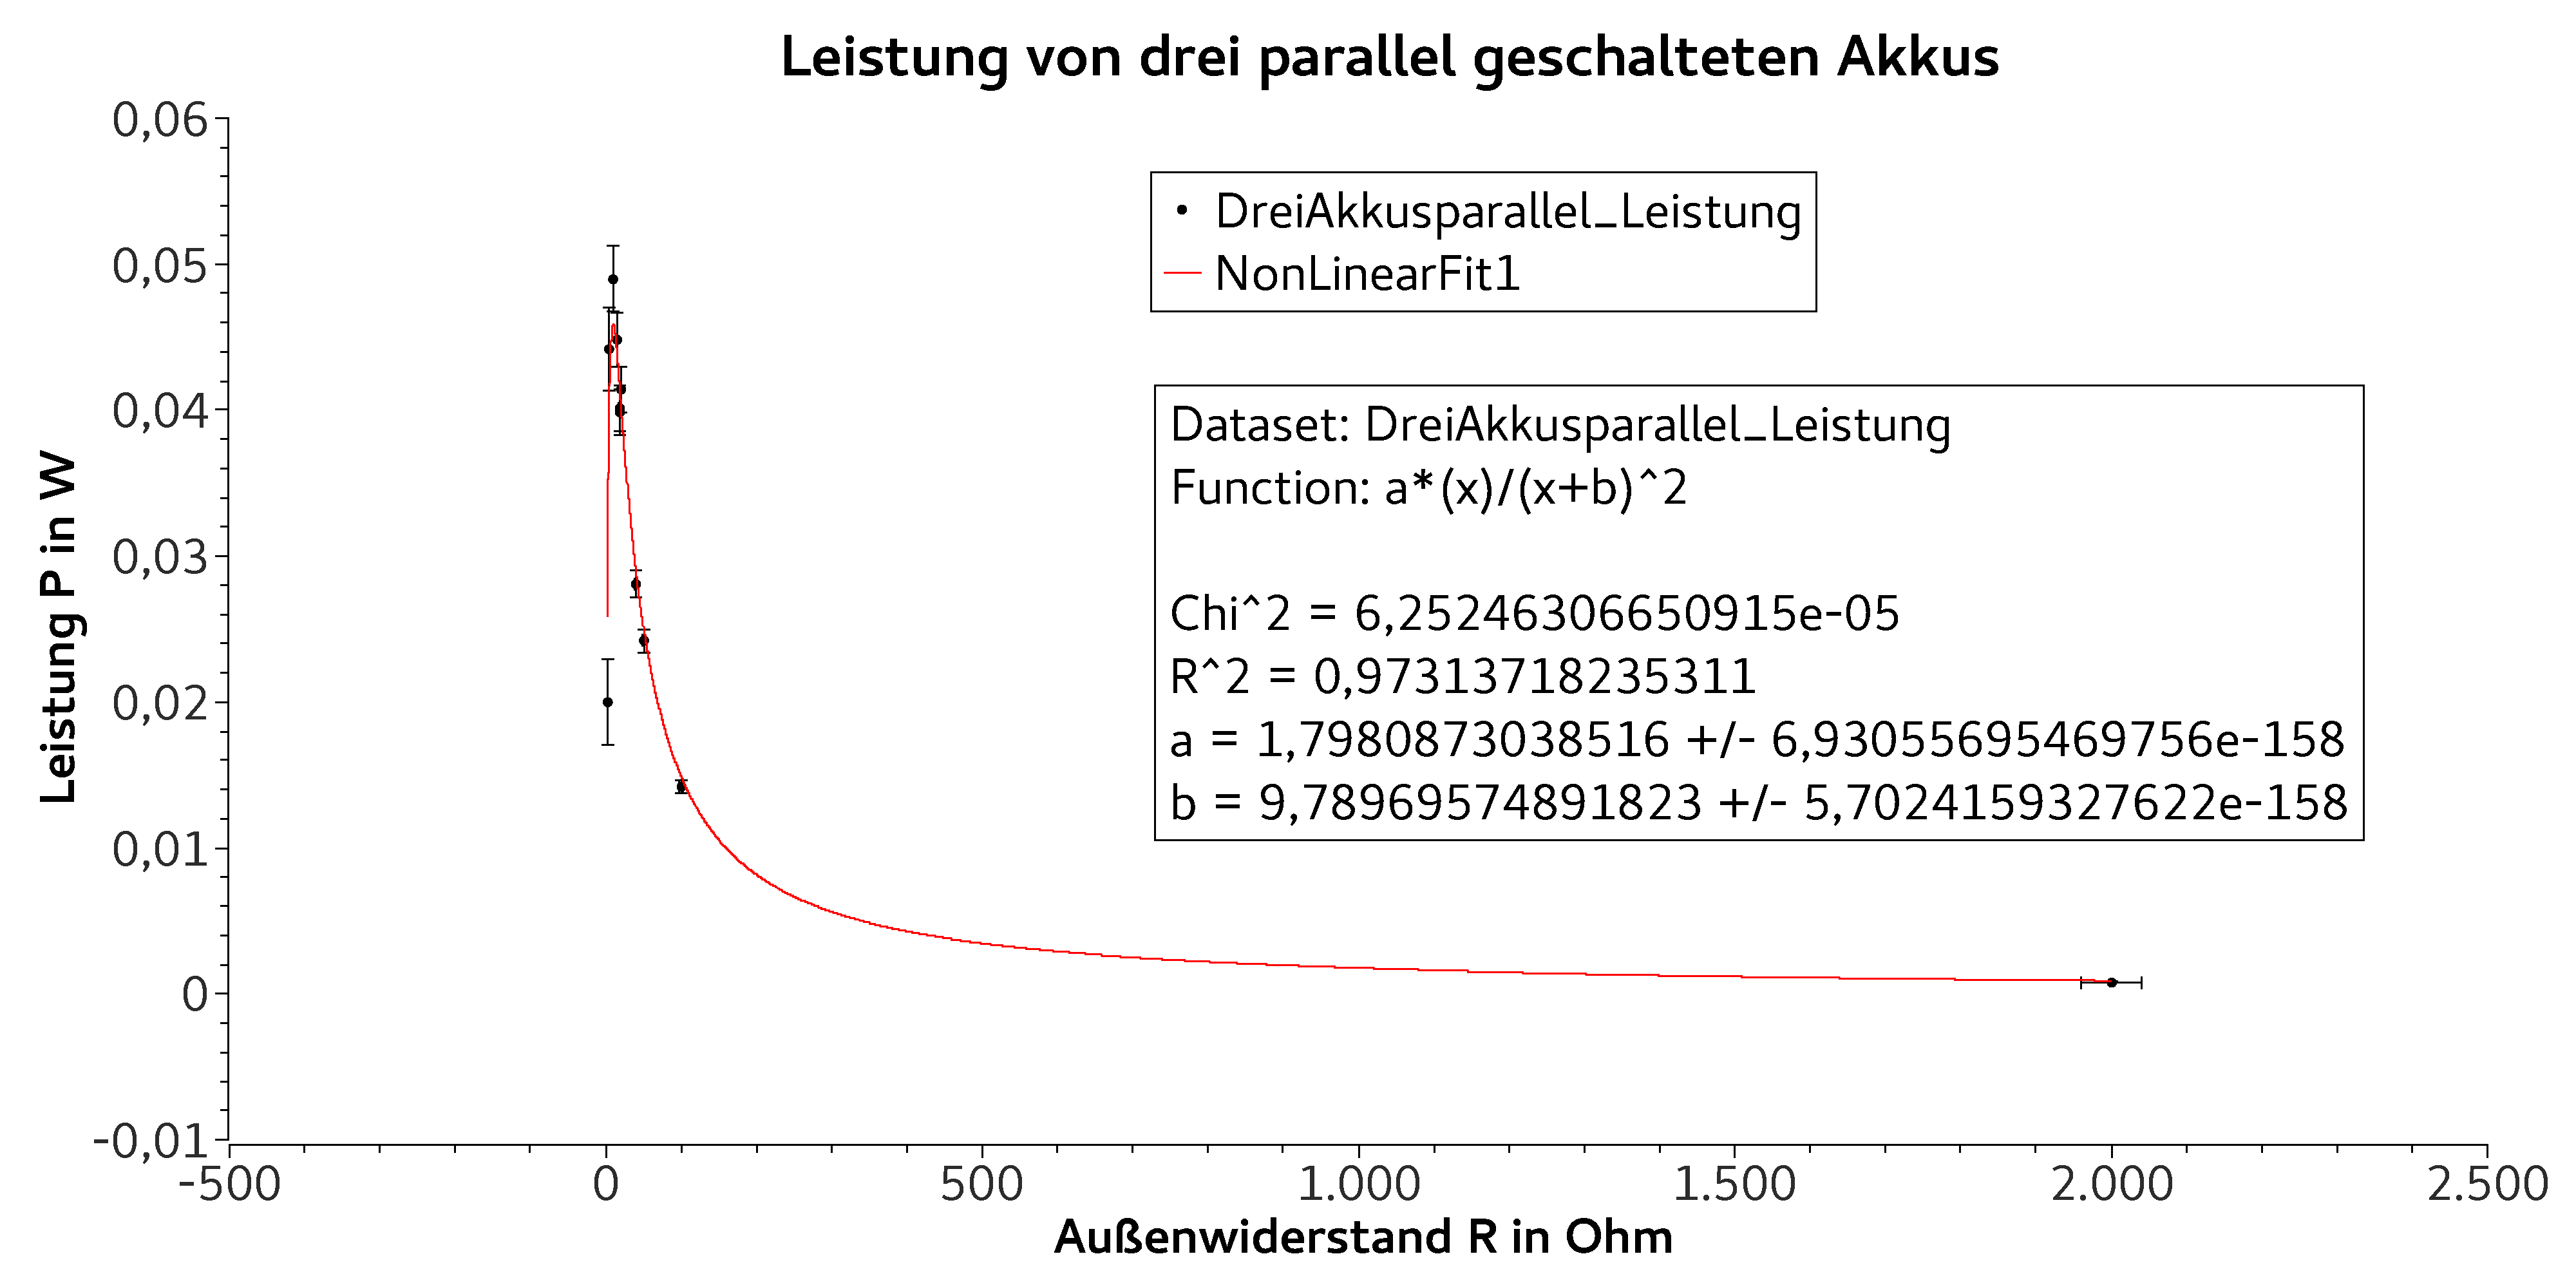
\includegraphics[width=1\textwidth]{Leistung3Parallel}
		\centering
		\caption{Die gemessene Leistung bei drei parallelen Akkus ist gegen den Außenwiderstand aufgetragen.}
		\label{Leistung3Parallel}
		\centering
	\end{figure}

	\subsubsection{Gleich- und Wechselstrom mit verschiedenen Verbrauchern}
	\subsubsection*{Widerstand}
	%TODO Satz das das hgicht tech plastik/metall ding verlustfrei ist
	In \cref{WiderSpannungGleich} und \cref{WiderSpannungWechsel} wurde die Spannung über einem Widerstand gegen den Strom aufgetragen. 
	Die Steigung der linearen Fits entspricht dem Widerstand $R = \SI{15,72 \pm 0,04}{\Omega}$ bzw. $\SI{15,55 \pm 0,04}{\Omega}$. 
	Der verwendete Widerstand wurde grob anhand der Einstellung des Potentiometers abgelesen, was \SI{14 \pm 1,7}{\Omega} ergab.
	Hierfür wurde vorausgesetzt, dass der Widerstand mit dem Drehungsgrad des Potentiometerdrehknopfes linear steigt.
	Dies kann aufgrund der Bauweise des Potentiometers so angenommen werden.

	In \cref{WiderLeistungGleich} und \cref{WiderLeistungWechsel} ist die Leistung gegen das Produkt von Strom und Spannung über den Widerstand aufgetragen. 
	Es ist in beiden Fällen eine Steigung von 1 zu erwarten, da $P = UI$ gilt. 
	Im Fall des Wechselstroms wurden nur Effektivwerte gemessen. 
	Da dies einen Faktor von $\frac{1}{2}$ für die Leistung und 2 Faktoren von $\sqrt{2}$ für $UI$ bedeutet, bleibt die Steigung dieselbe.
	Die Steigung der linearen Fits betragen jedoch \SI{0,775 \pm 0,004}{} und \SI{0,787 \pm 0,005}{}.
	\begin{figure}[tb]
		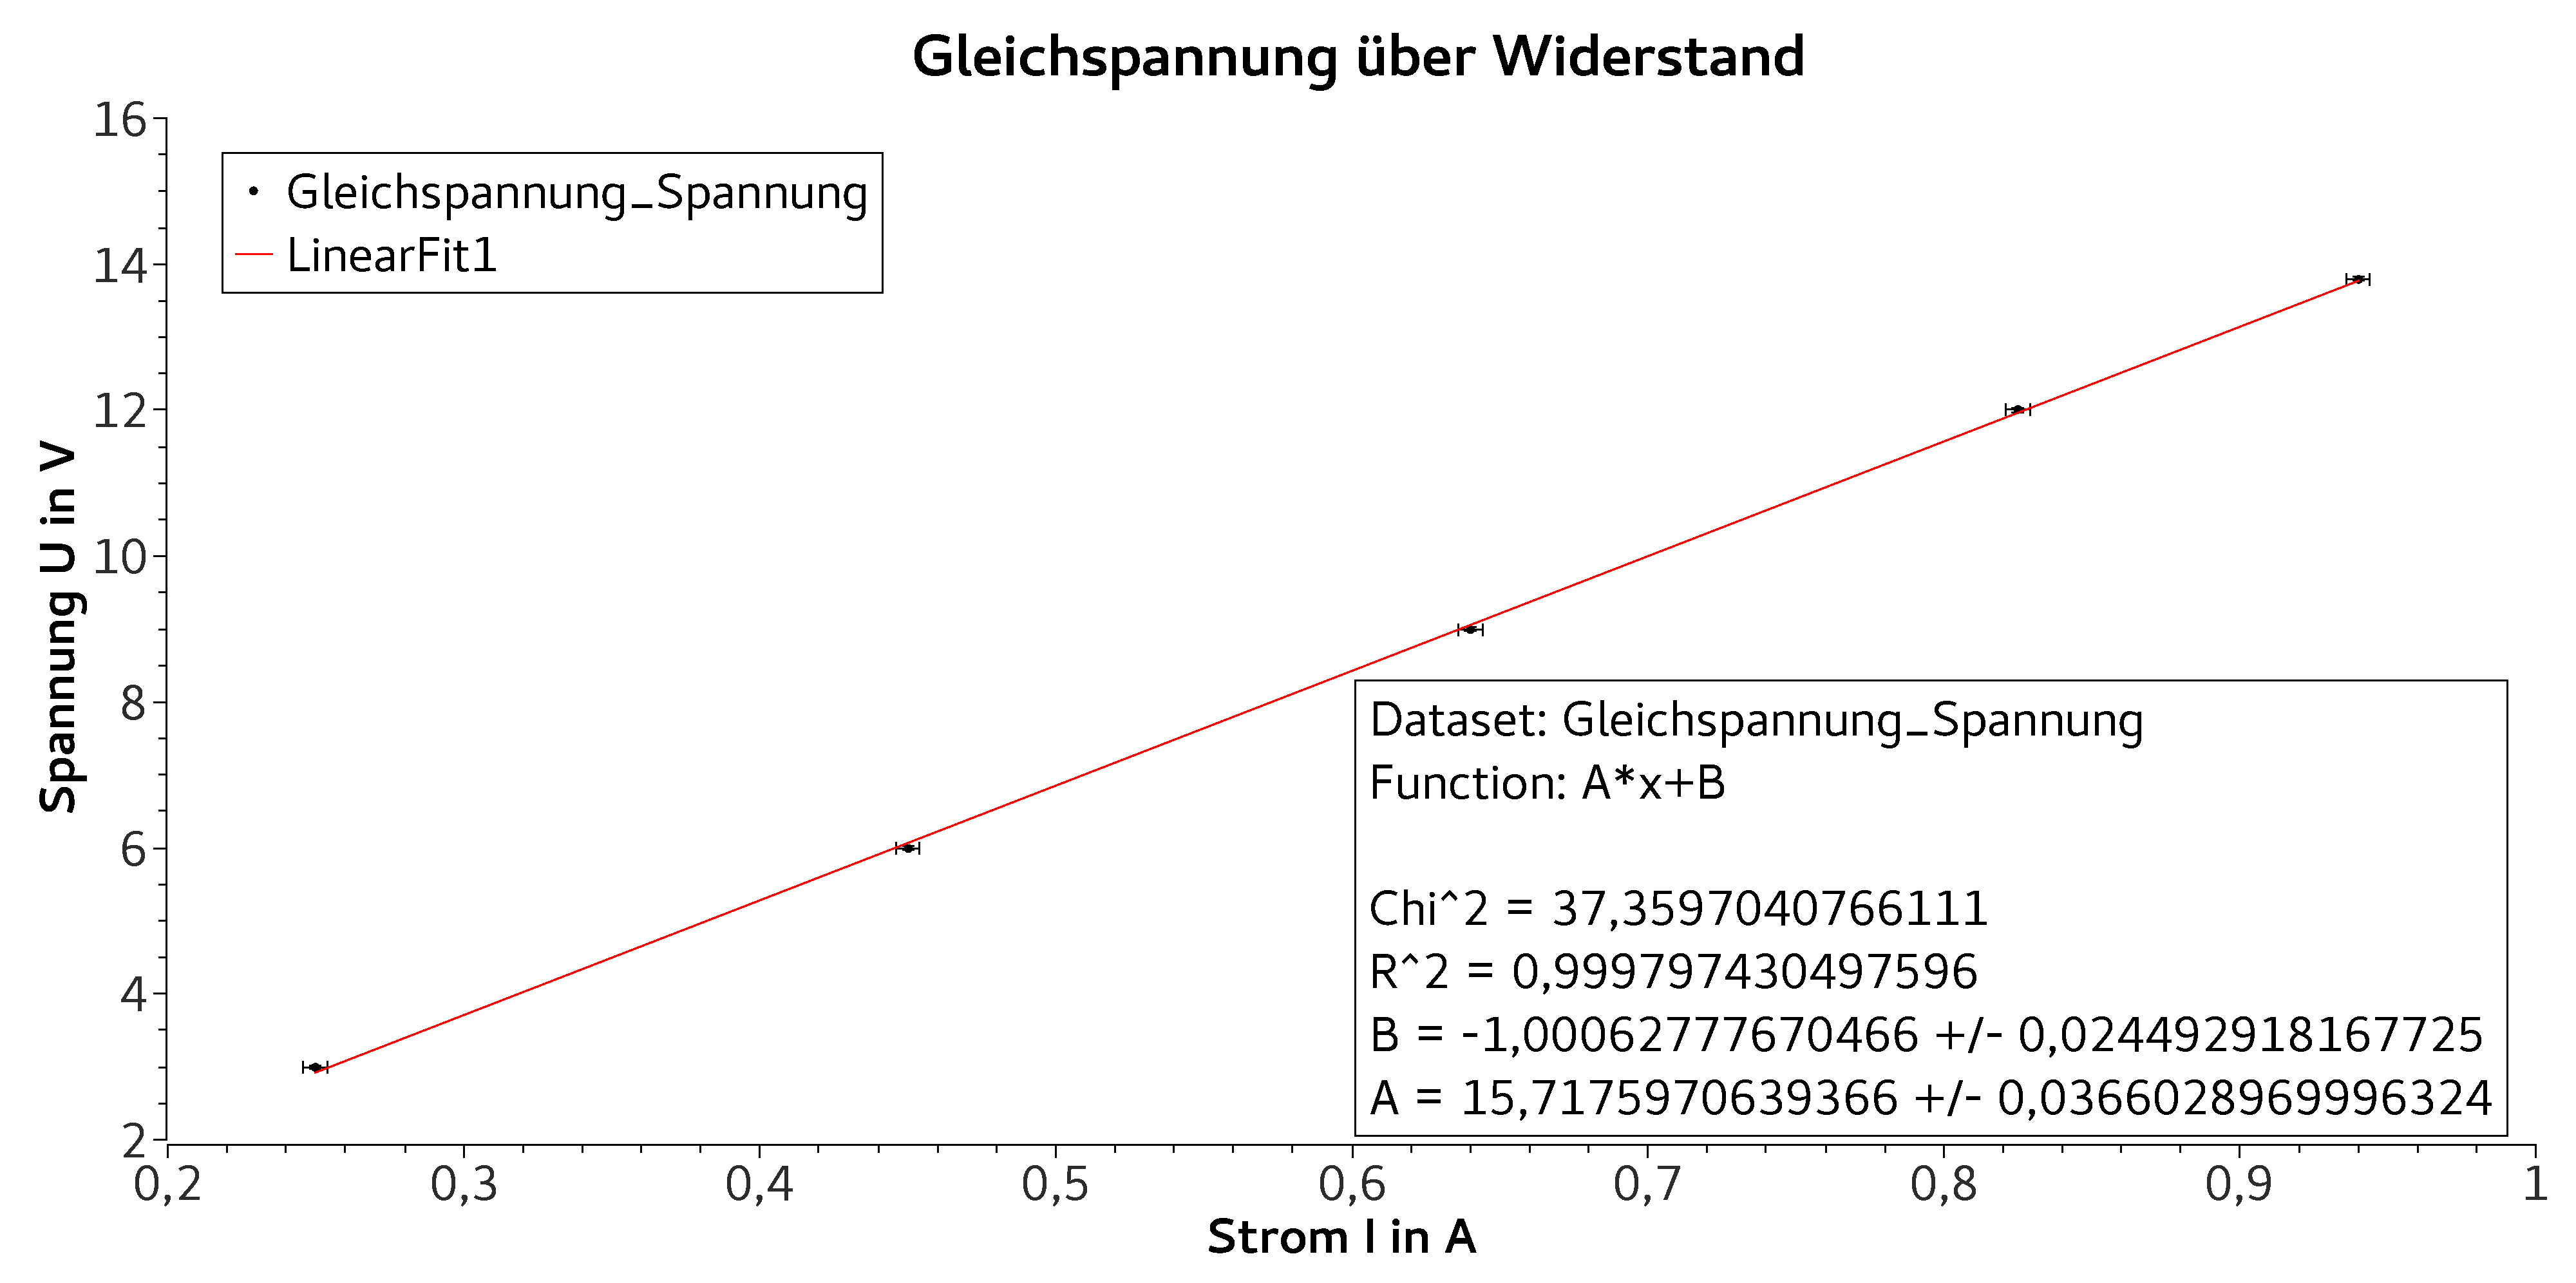
\includegraphics[width=1\textwidth]{WiderSpannungGleich}
		\centering
		\caption{Die gemessene Gleichspannung über einen Widerstand ist gegen den Gleichstrom aufgetragen.}
		\label{WiderSpannungGleich}
		\centering
	\end{figure}
	\begin{figure}[tb]
		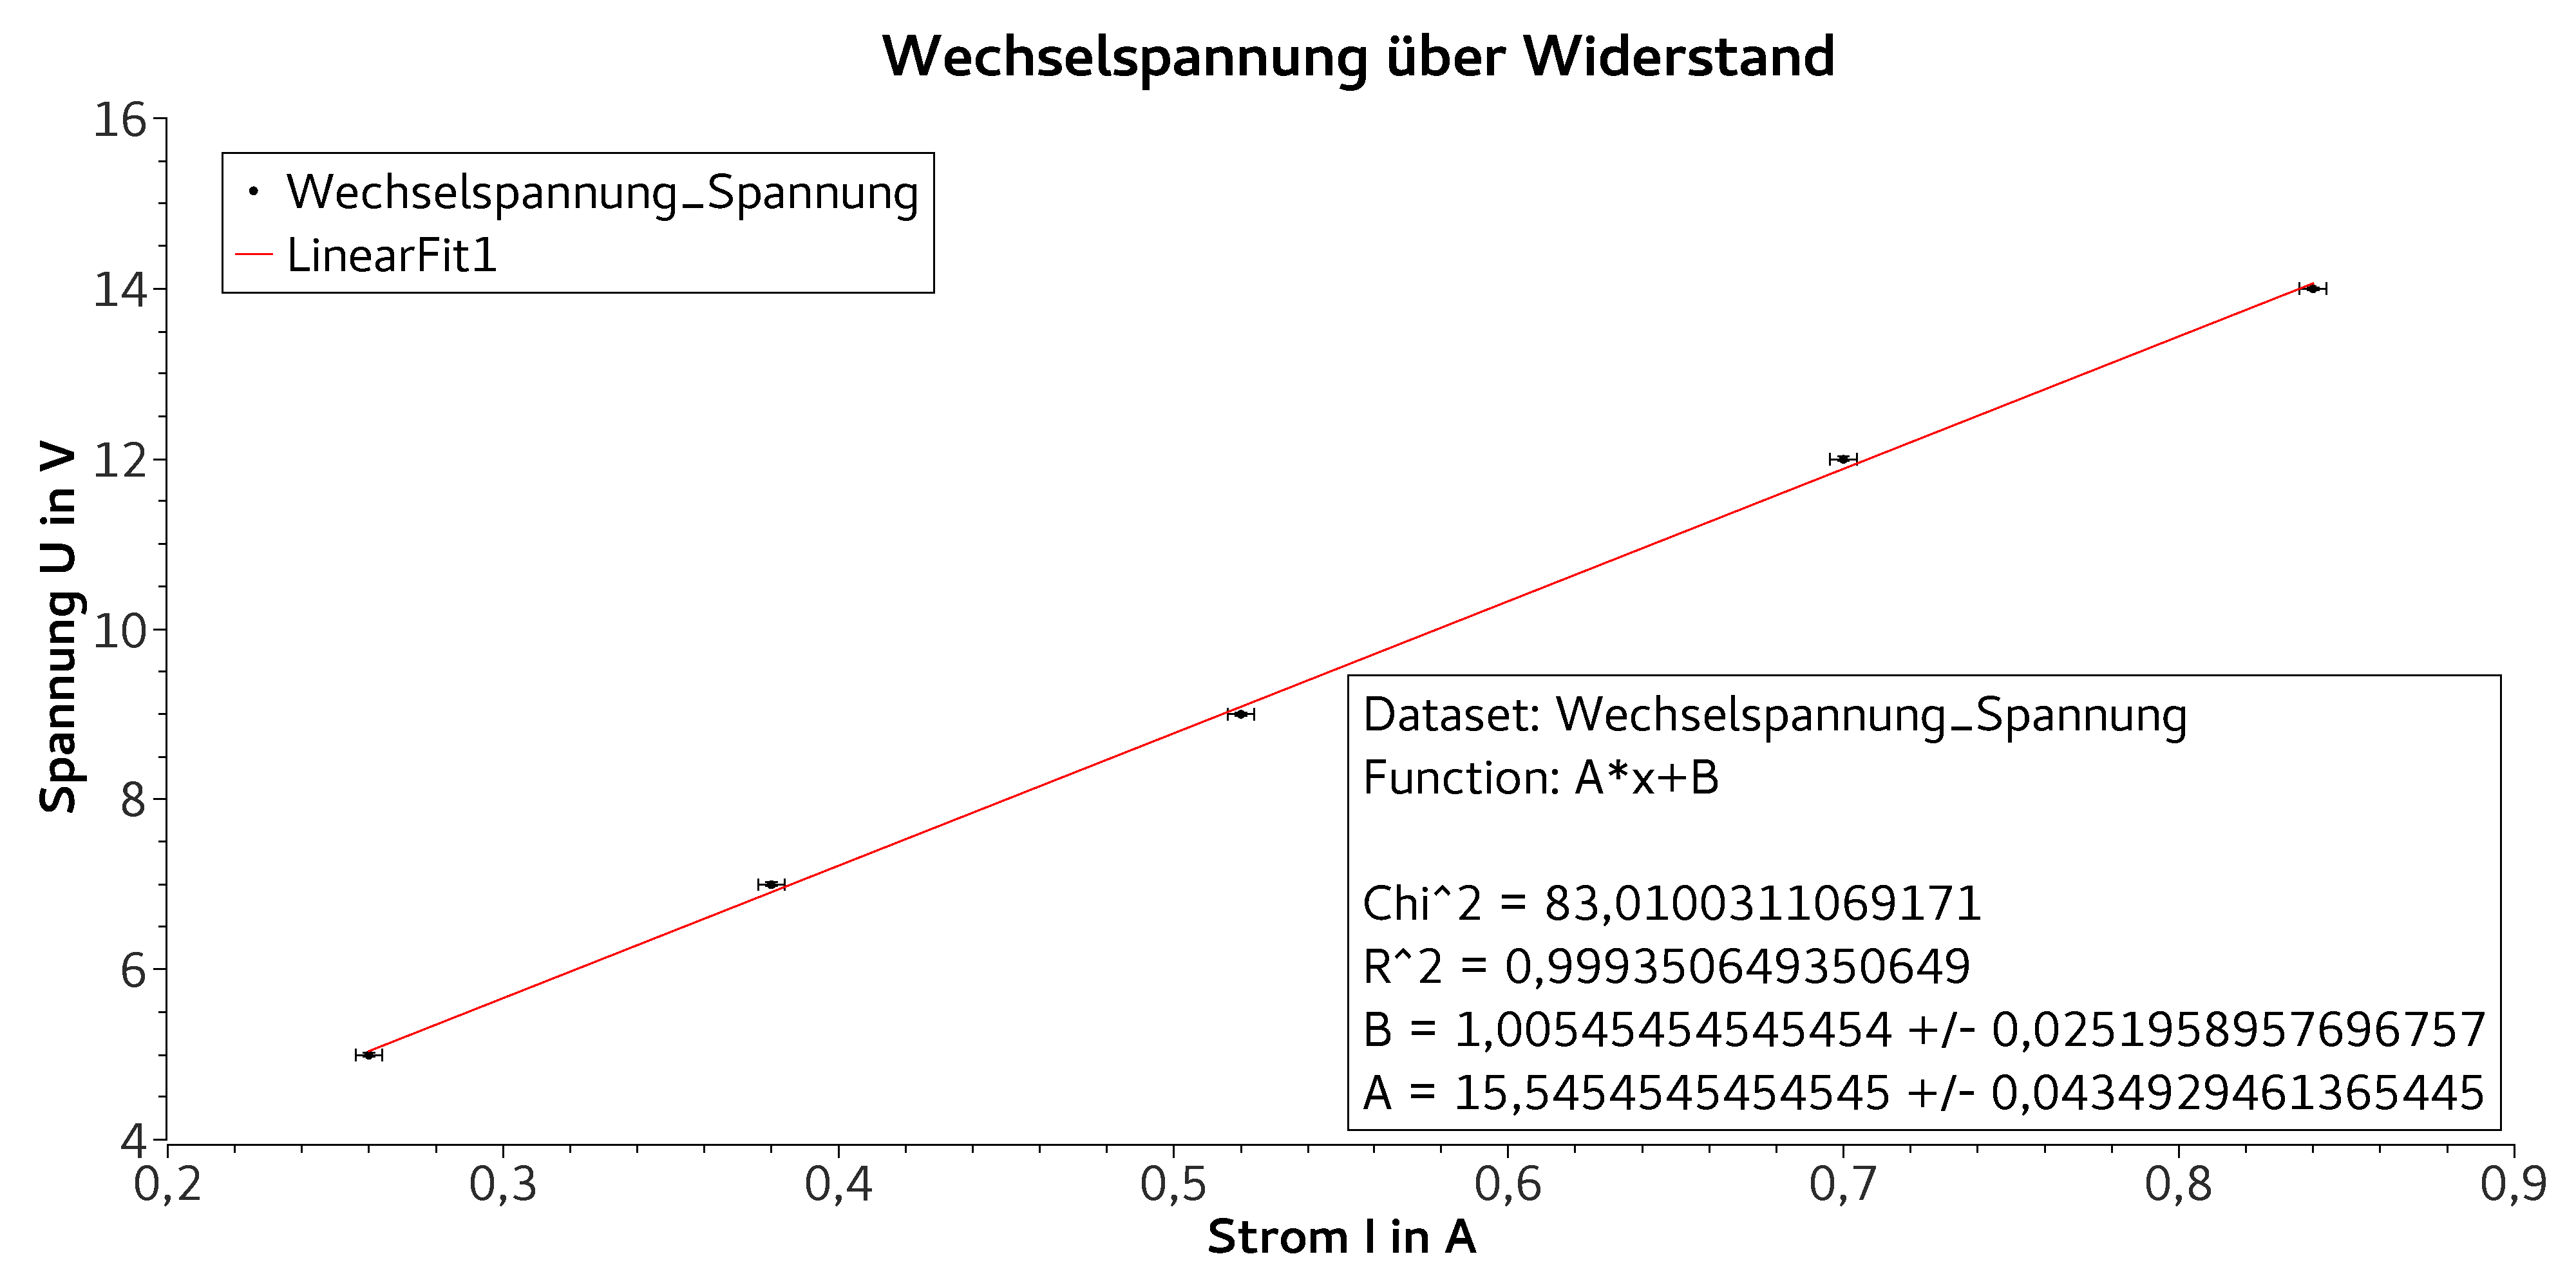
\includegraphics[width=1\textwidth]{WiderSpannungWechsel}
		\centering
		\caption{Die gemessene effektive Wechselspannung über einen Widerstand ist gegen den effektiven Wechselstrom aufgetragen.}
		\label{WiderSpannungWechsel}
		\centering
	\end{figure}

	\begin{figure}[tb]
		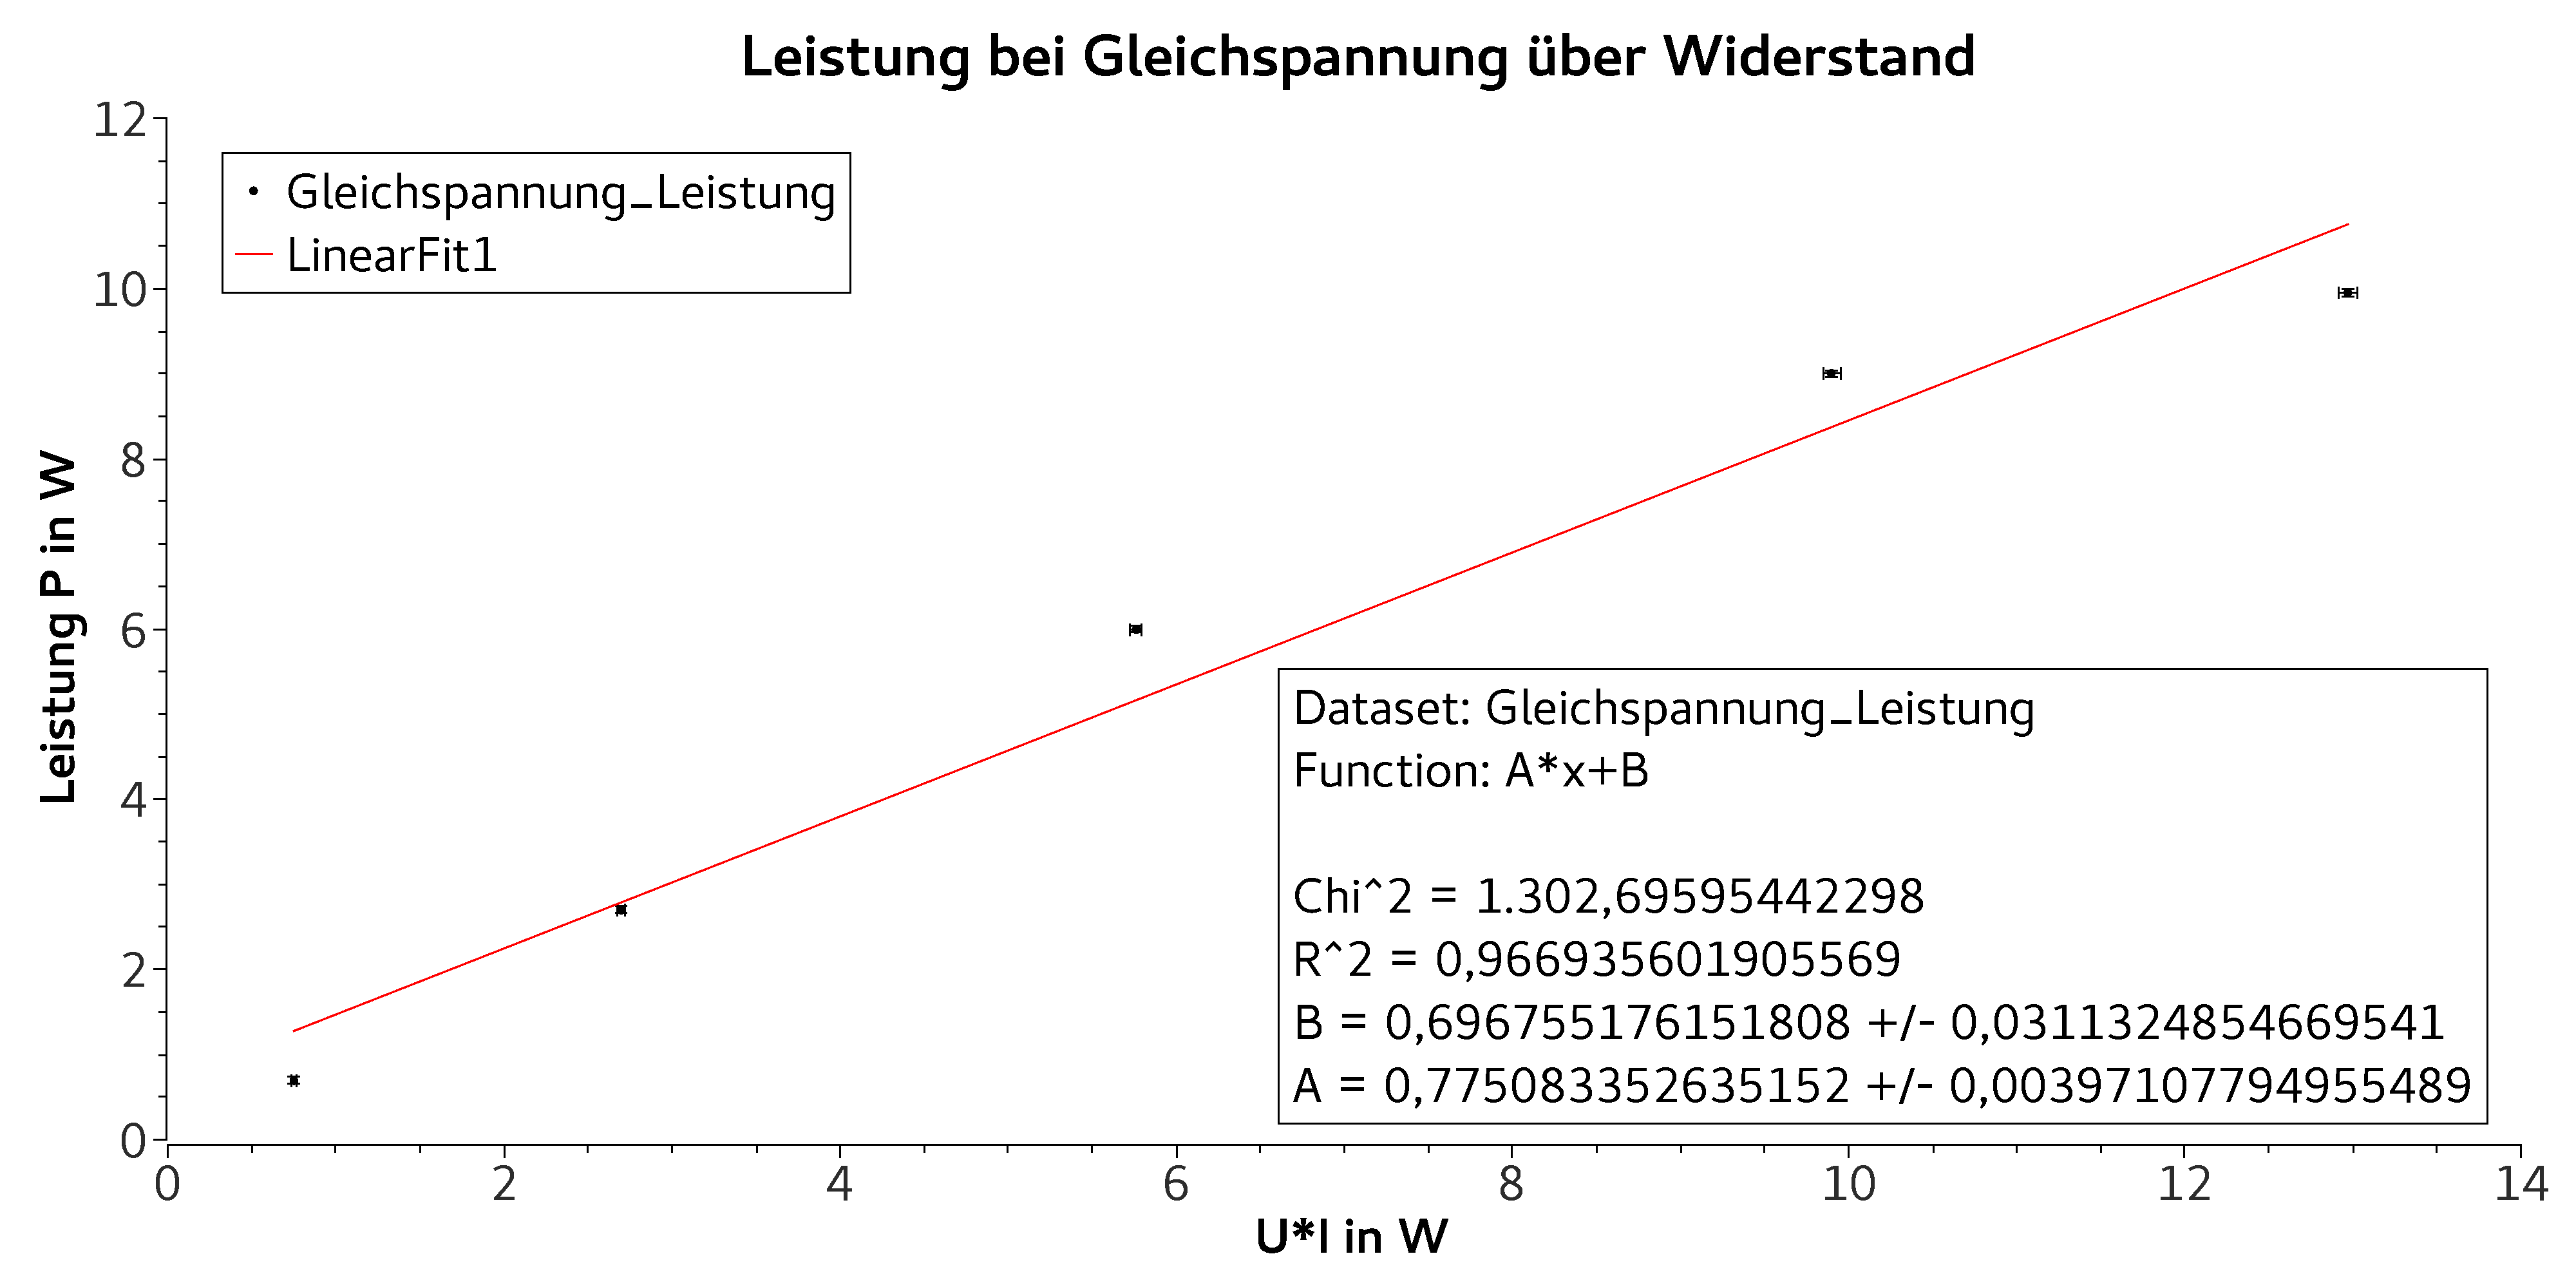
\includegraphics[width=1\textwidth]{WiderLeistungGleich}
		\centering
		\caption{Die gemessene Leistung ist gegen das Produkt aus Gleichstrom und Gleichspannung über einen Widerstand aufgetragen.} 
		\label{WiderLeistungGleich}
		\centering
	\end{figure}
	
	\begin{figure}[tb]
		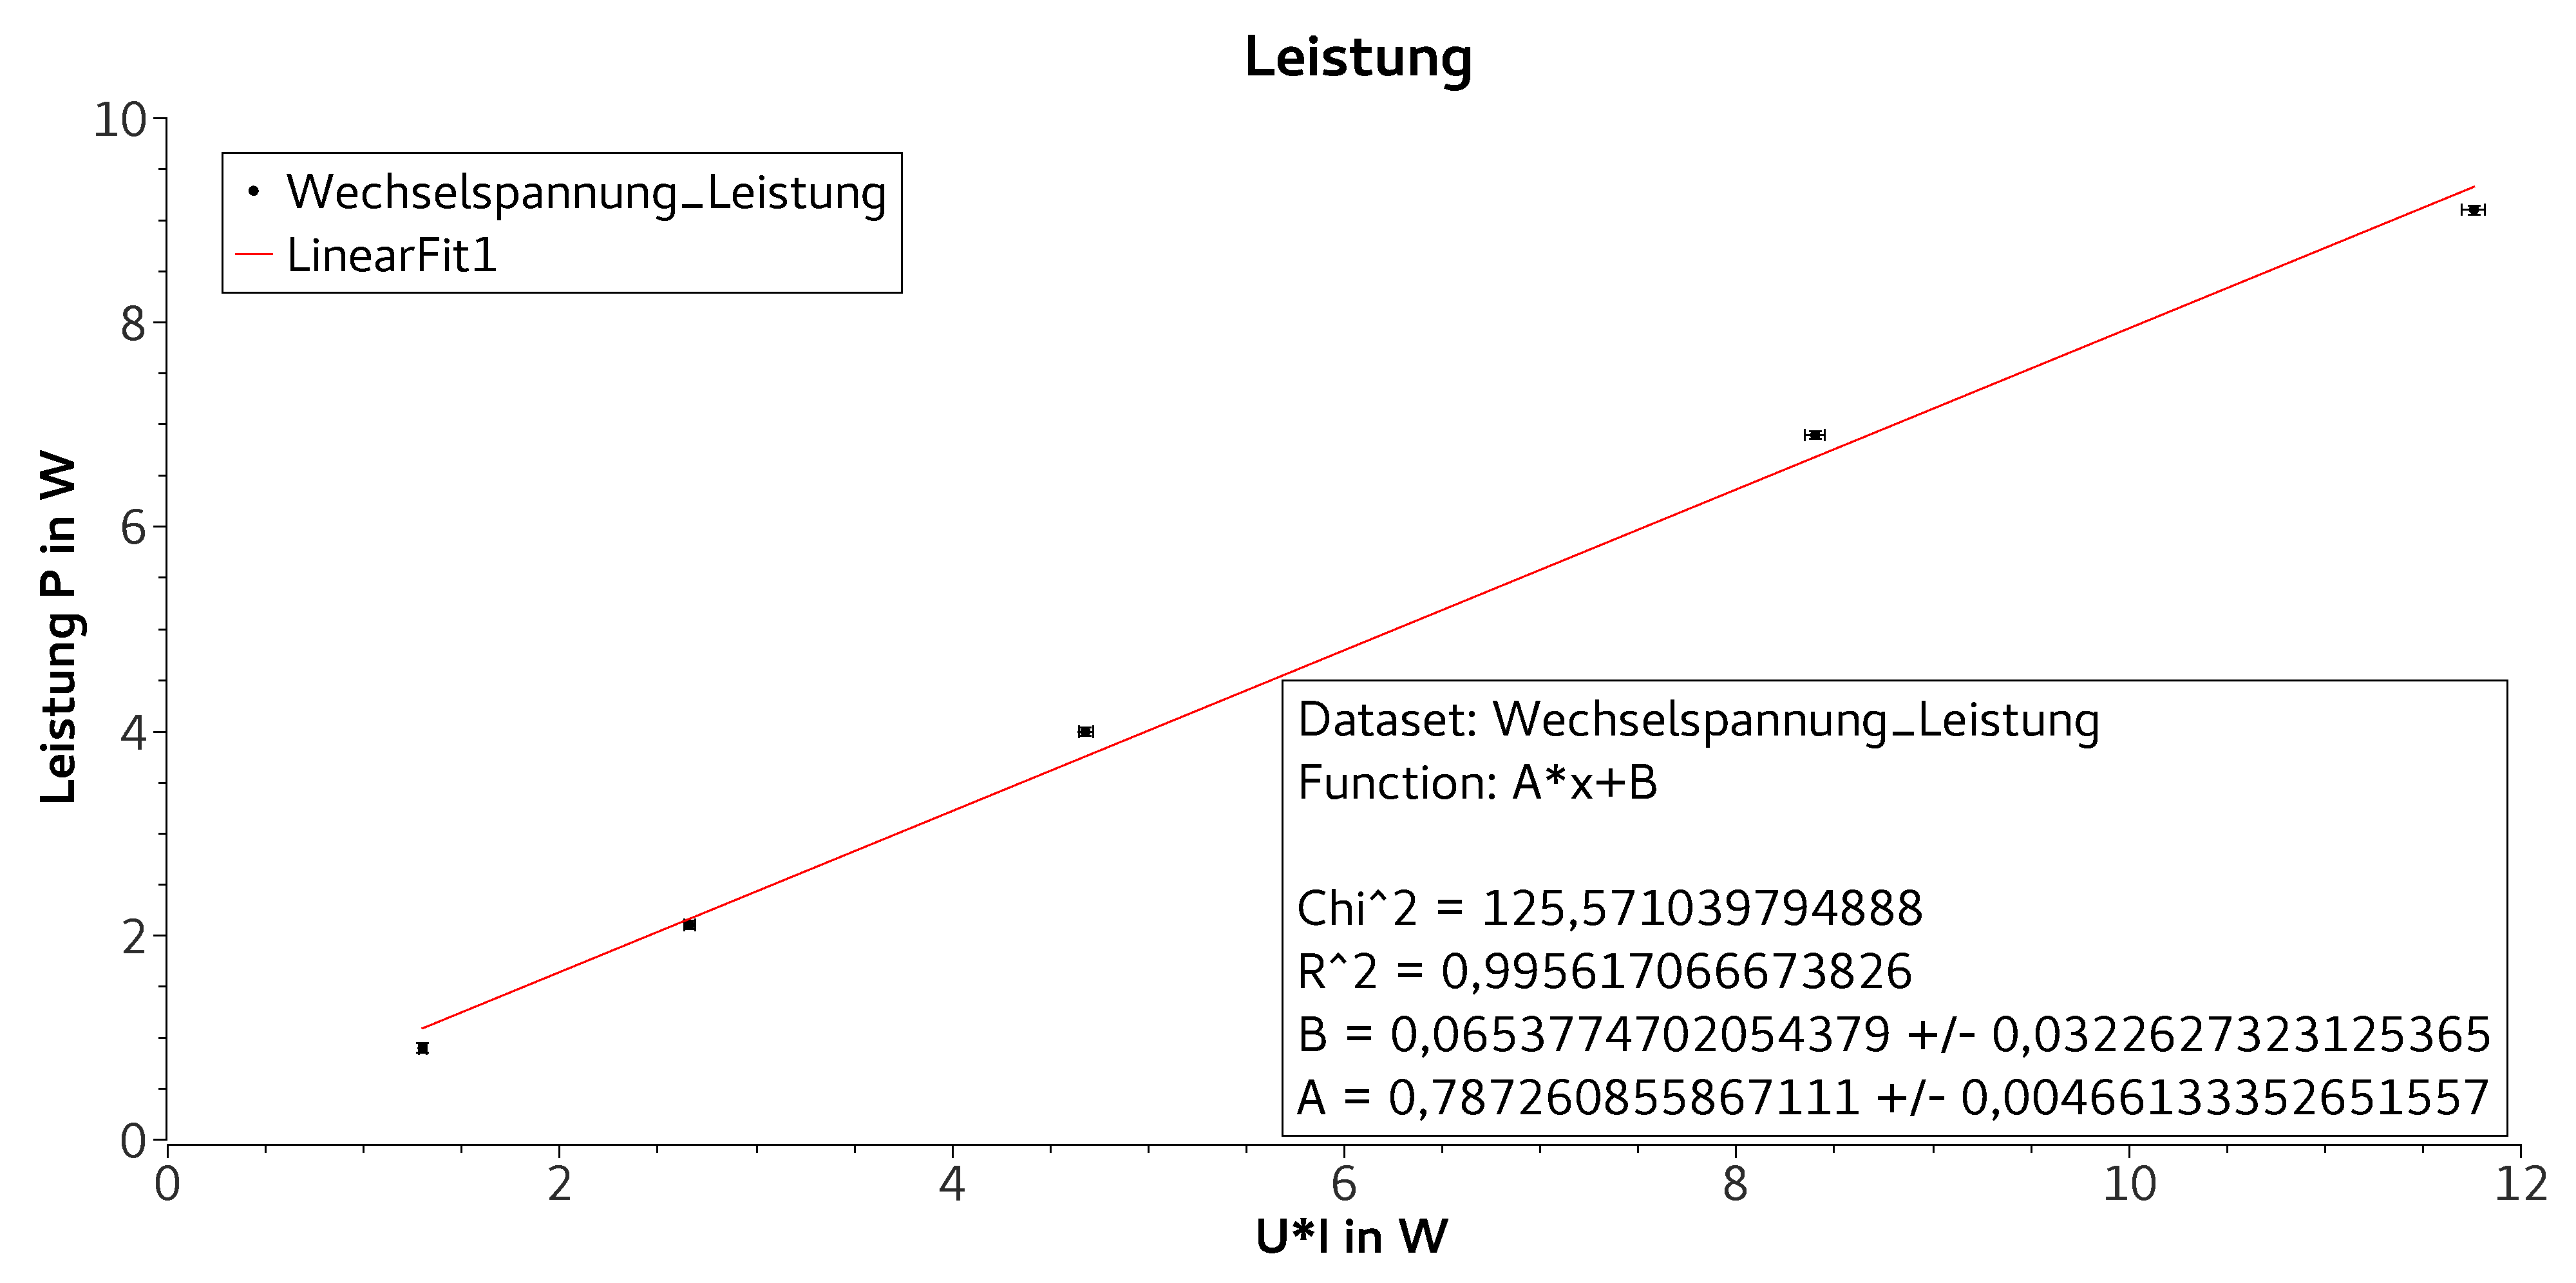
\includegraphics[width=1\textwidth]{WiderLeistungWechsel}
		\centering
		\caption{Die gemessene effektive Leistung ist gegen das Produkt aus effektivem Wechselstrom und effektiver Wechselspannung über einen Widerstand aufgetragen.}
		\label{WiderLeistungWechsel}
		\centering
	\end{figure}

	\subsubsection*{Spule}
	Die gemessene effektive Wechselspannung über die Spule ist gegen den effektiven Strom in \cref{SpuleSpannungWechsel} aufgetragen.
	Die Steigung des linearen Fits ist der Scheinwiderstand $|Z|$ $\SI{30,00 \pm 0,06}{\Omega}$. 
	
	Der Widerstand der Spule findet sich in \cref{SpuleSpannungGleich} wieder. 
	In diesem Graphen wurde die Gleichspannung über die Spule gegen den Gleichstrom aufgetragen und analog ist die Steigung des Fits der Innenwiderstand $R_\text{i}$ $\SI{24,04 \pm 0,06}{\Omega}$.

	Aus der Theorie ist folgender Zusammenhang bekannt:
	\begin{equation}
		\bar{P} = U_\text{eff} I_\text{eff} \cos(\phi)
	\end{equation}
	\cref{SpuleLeistungWechsel} beinhaltet die Messwerte für die effektive Leistung in Abhängigket von dem Produkt der effektiven Spannung und des effektiven Stroms. 
	Der linearer Fit hat die Steigung $\SI{0,7965\pm 0,0041}{}$, was $\cos(\phi)$ entsprechen sollte. 
	Es folgt also ein $\phi$ von $\ang{37,202\pm 0,385}$.

	Die Indukivität der Spule lässt sich durch die bereits bestimmten Werte und \cref{Spule} bestimmen.
	\begin{gather}
		\label{Spule}
		|Z| = \sqrt{R_\text{W}^2 + (\omega L)^2} \\
		L = \frac{1}{\omega}\sqrt{|Z|^2-R_\text{W}^2} \\
		R_\text{W} = |Z| \cos(\phi)  \\
		L = \frac{1}{\omega} \sin{\phi} |Z|
	\end{gather}
		Das Stromnetz hat eine Frequenz von \SI{50}{Hz}. 
		Diese kann als exakt angenommen werden, da im deutschen Stromnetz die Frequenz sehr präzise geregelt wird und die Schwankung hier gegenüber den anderen Fehlern verschwinden würde.
		Es ergibt sich ein Wirkwiderstand von \SI{23,90 \pm 0,06}{\Omega}.
		Daraus folgt eine Induktivität von \SI{0,0577 \pm 0,00019}{H}. 
	

	\begin{figure}[tb]
		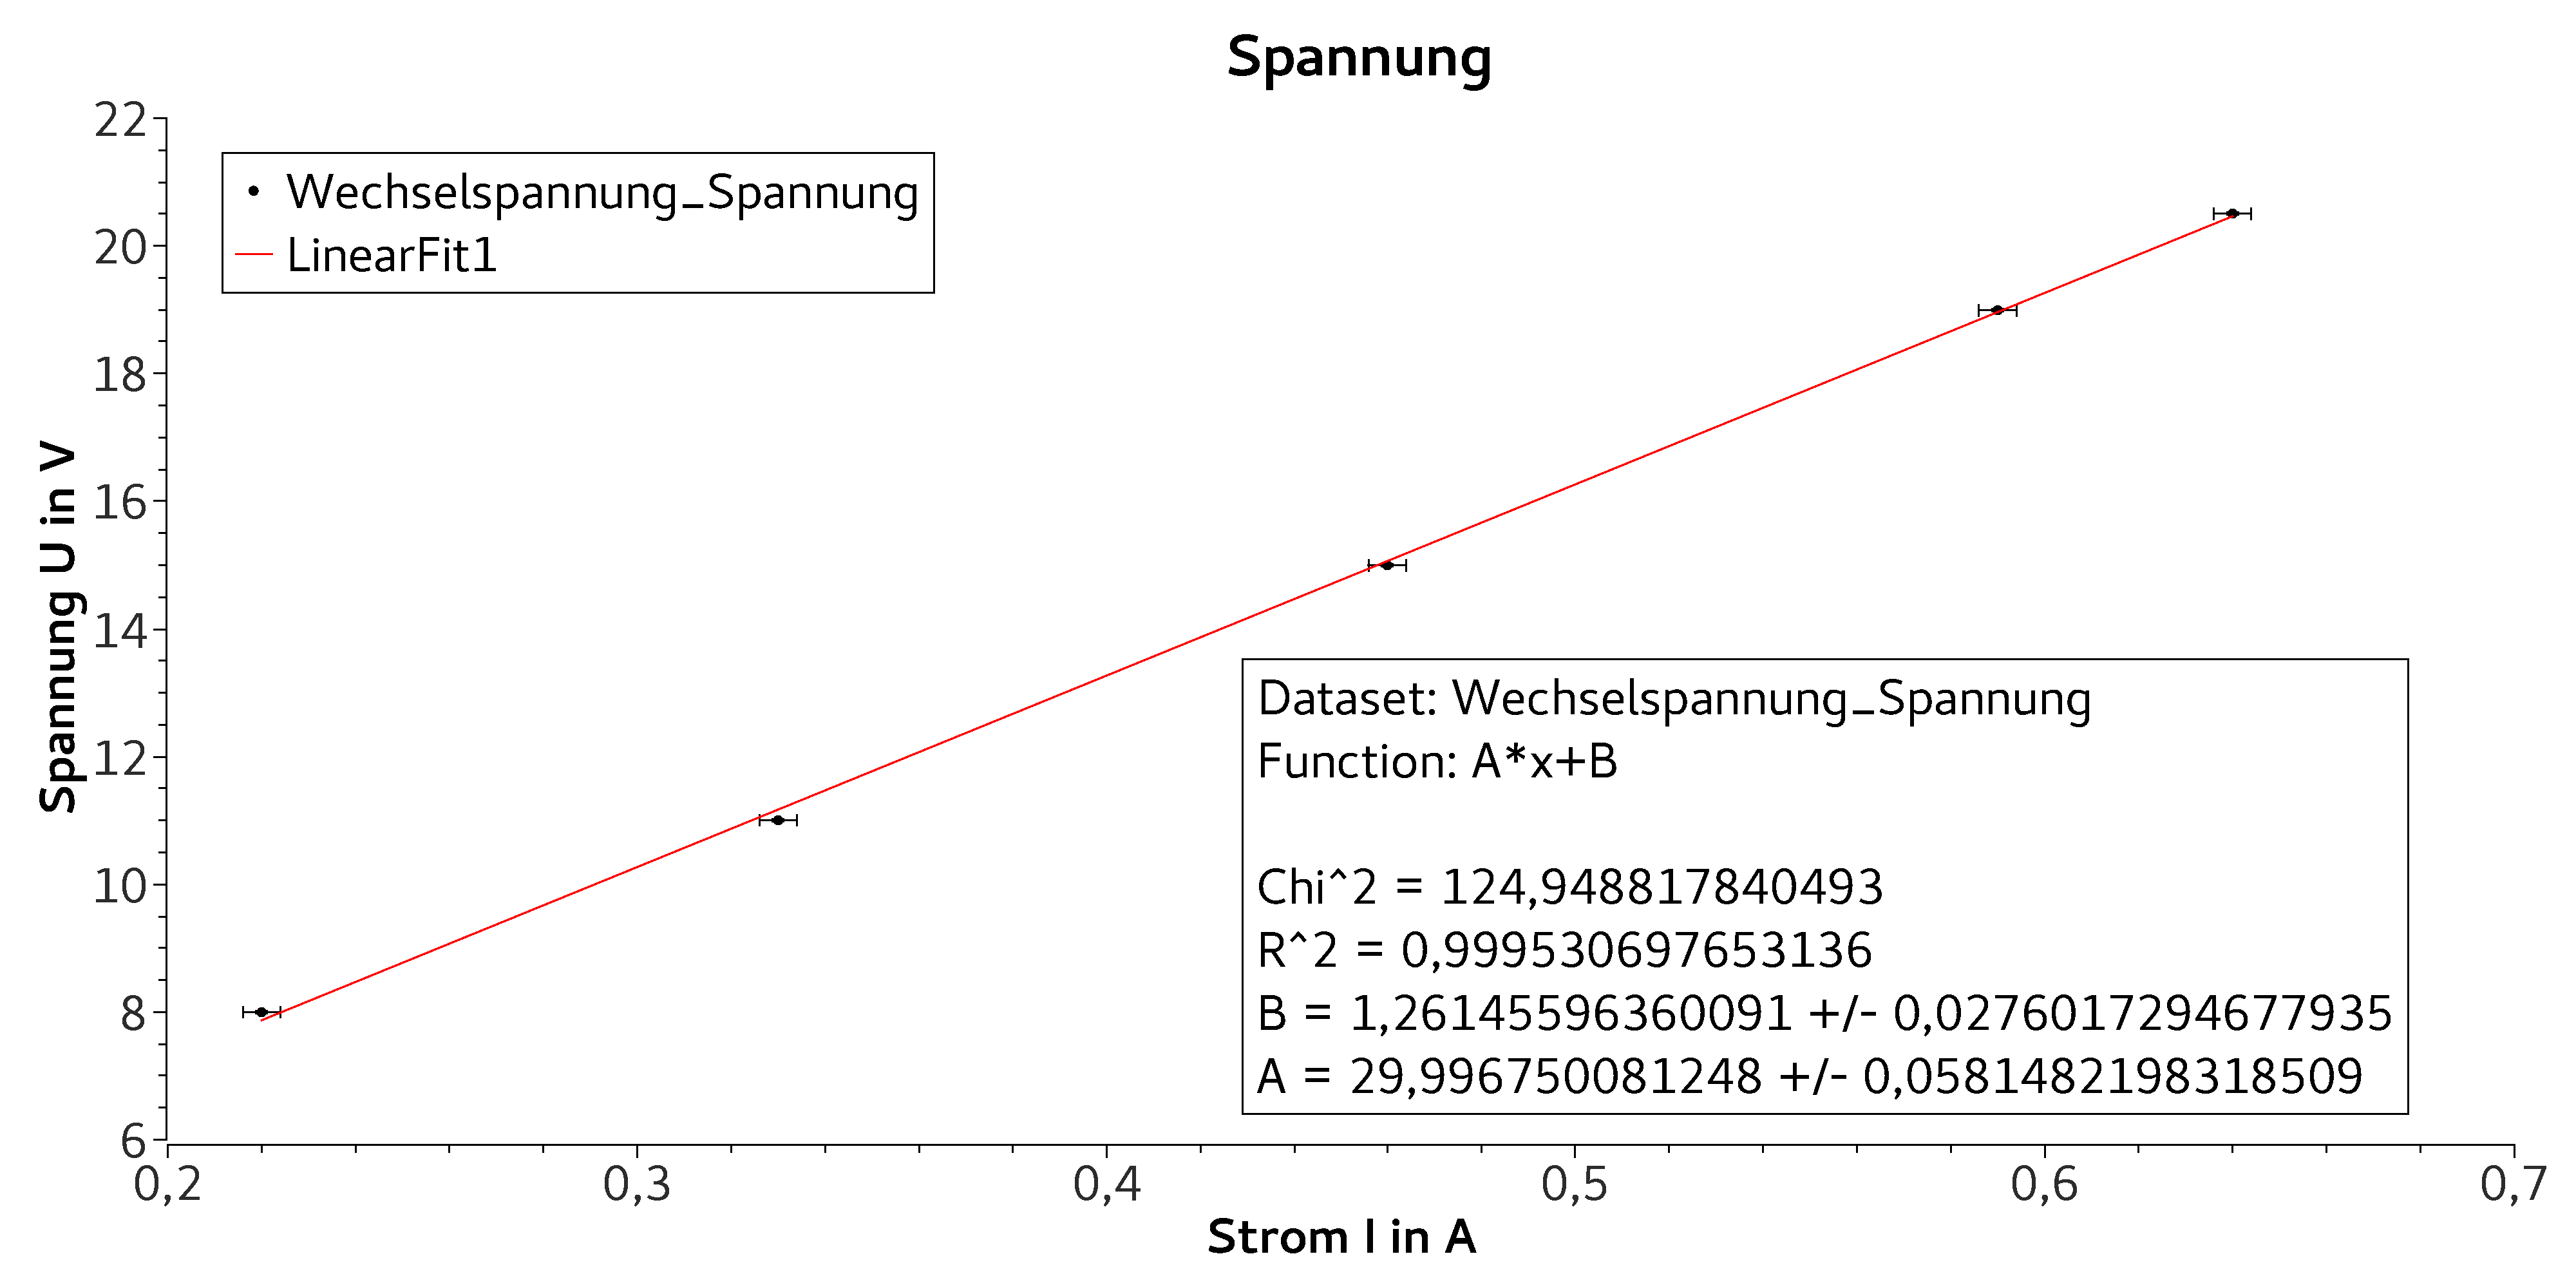
\includegraphics[width=1\textwidth]{SpuleSpannungWechsel}
		\centering
		\caption{Die gemessene effektive Wechselspannung über eine Spule ist gegen den effektiver Wechselstrom aufgetragen.}
		\label{SpuleSpannungWechsel}
		\centering
	\end{figure}
	\begin{figure}[tb]
		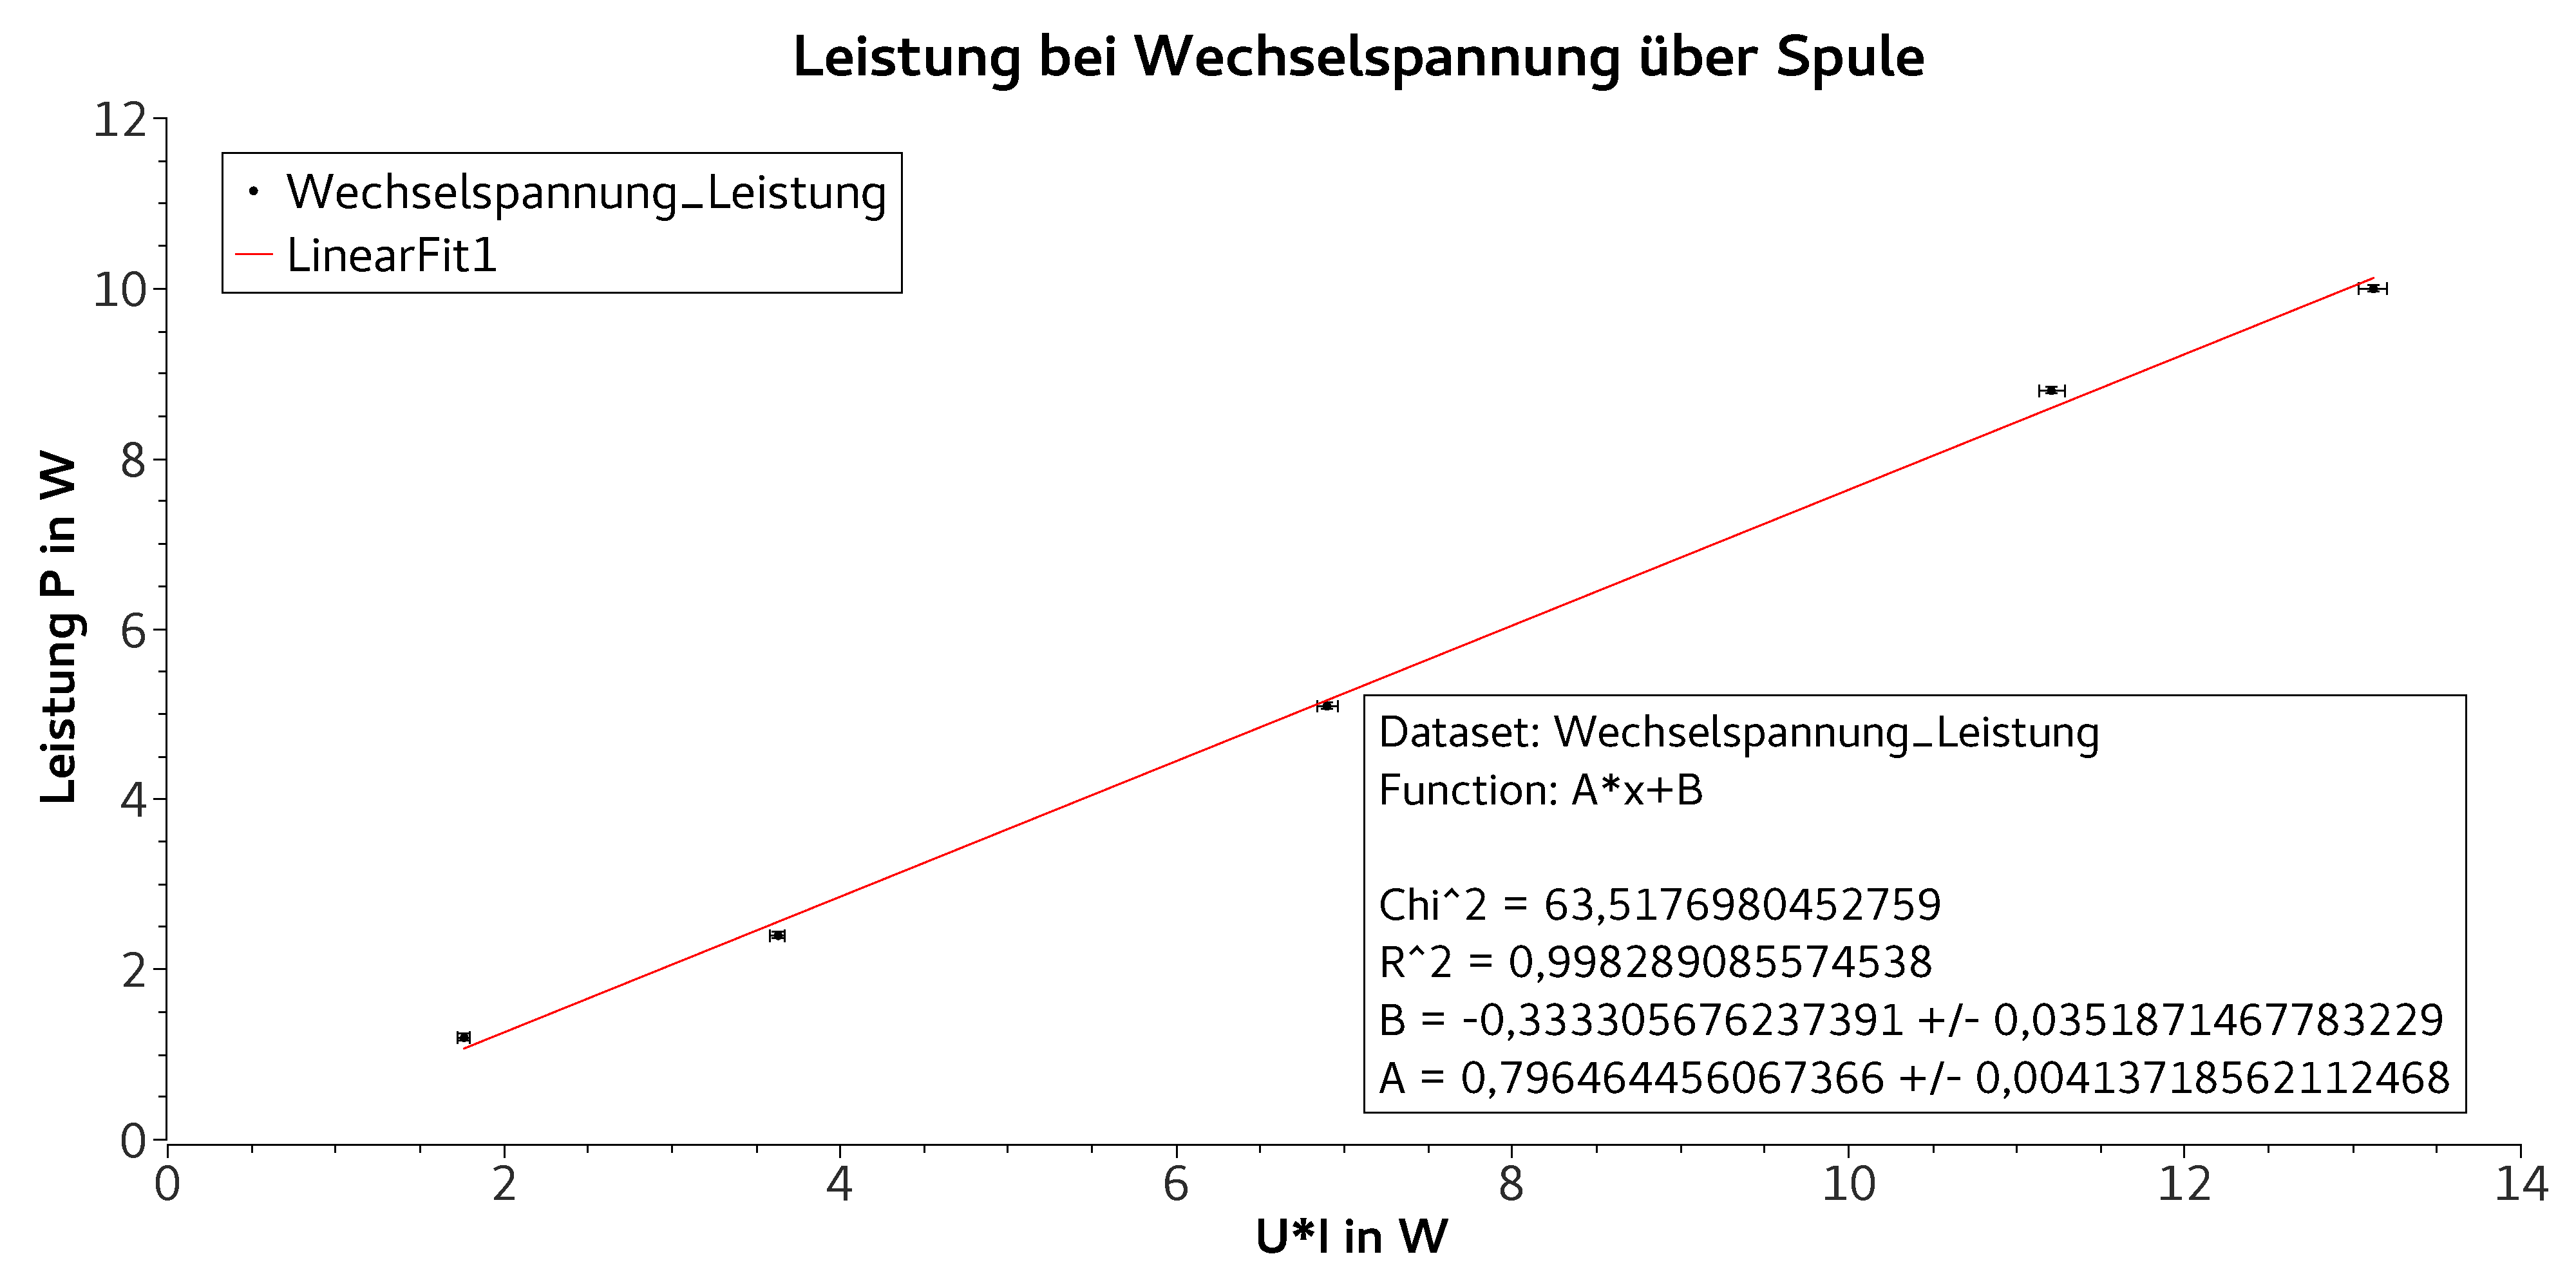
\includegraphics[width=1\textwidth]{SpuleLeistungWechsel}
		\centering
		\caption{Die gemessene effektive Leistung ist gegen das Produkt aus Wechselstrom und Wechselspannung über eine Spule aufgetragen.}
		\label{SpuleLeistungWechsel}
		\centering
	\end{figure}
	\begin{figure}[tb]
		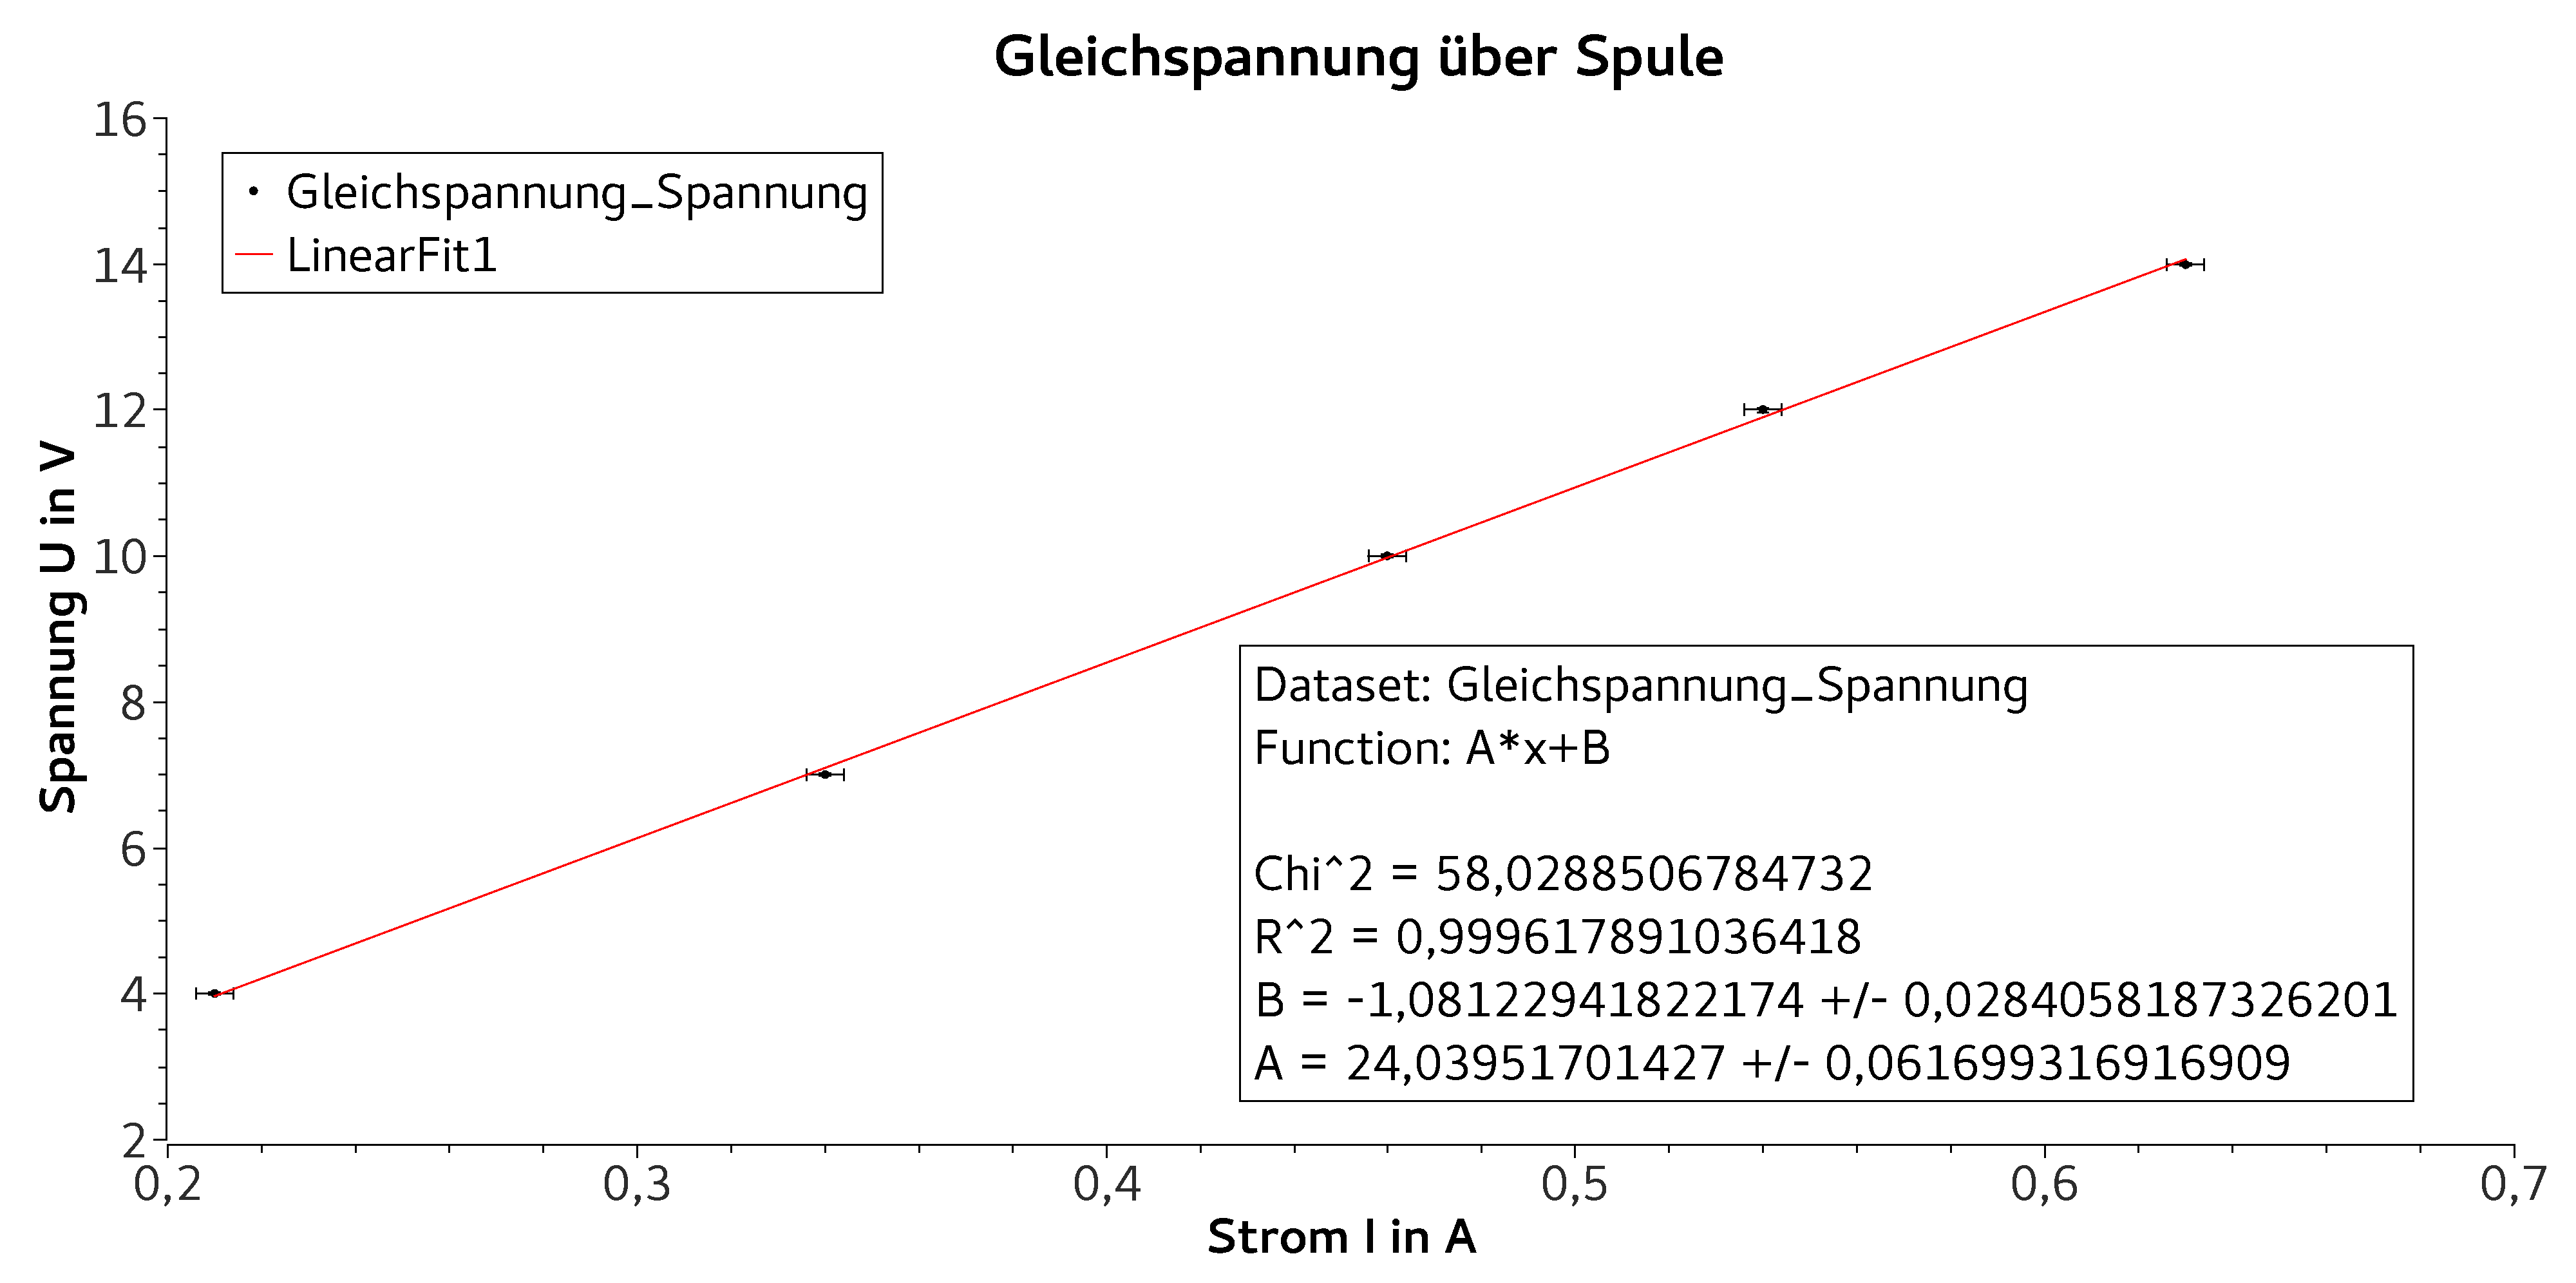
\includegraphics[width=1\textwidth]{SpuleSpannungGleich}
		\centering
		\caption{Die gemessene Spannung über eine Spule ist gegen den Strom aufgetragen.}
		\label{SpuleSpannungGleich}
		\centering
	\end{figure}

	\subsubsection*{Spule und Kondensator in Reihe}
	Die gemessene effektive Wechselspannung über die Spule und den Kondensator ist gegen den effektiven Strom in \cref{KondensatorSpannungWechsel} aufgetragen.
	Die Steigung des linearen Fits ist der Betrag des Scheinwiderstandes $|Z|$ $\SI{41,81 \pm 0,07}{\Omega}$. 

	Aus der Theorie ist folgender Zusammenhang bekannt:
	\begin{equation}
		\bar{P} = U_\text{eff} I_\text{eff} \cos(\phi)
	\end{equation}
	\cref{KondensatorLeistungWechsel} beinhaltet die Messwerte für die effektive Leistung in Abhängigket von dem Produkt der effektiven Spannung und des effektiven Stroms. 
	Der linearer Fit hat die Steigung $\SI{0,651 \pm 0,004}{}$, was $\cos(\phi)$ entsprechen sollte. 
	Es folgt also ein $\phi$ von $-\ang{49,38 \pm 0,30}$.

	Die Kapaziät lässt sich mittels \cref{Kondensator} bestimmen.
	\begin{gather}
		\label{Kondensator}
		|Z| = \sqrt{R^2 + (\omega L - \frac{1}{\omega C})^2} \\
		C = \frac{1}{\omega^2 L- \omega\sqrt{Z^2-R^2}} \\
		C = \frac{1}{\omega^2 L- \omega|Z|\sin{\phi}} 
	\end{gather}
	Durch Einsetzten ergibt sich eine Kapazität $C$ von \SI{63,8 \pm 2,1}{\mu F}. Auf dem Kondensator war eine Kapazität von \SI{60}{\mu F} angegeben.




	\begin{figure}[tb]
		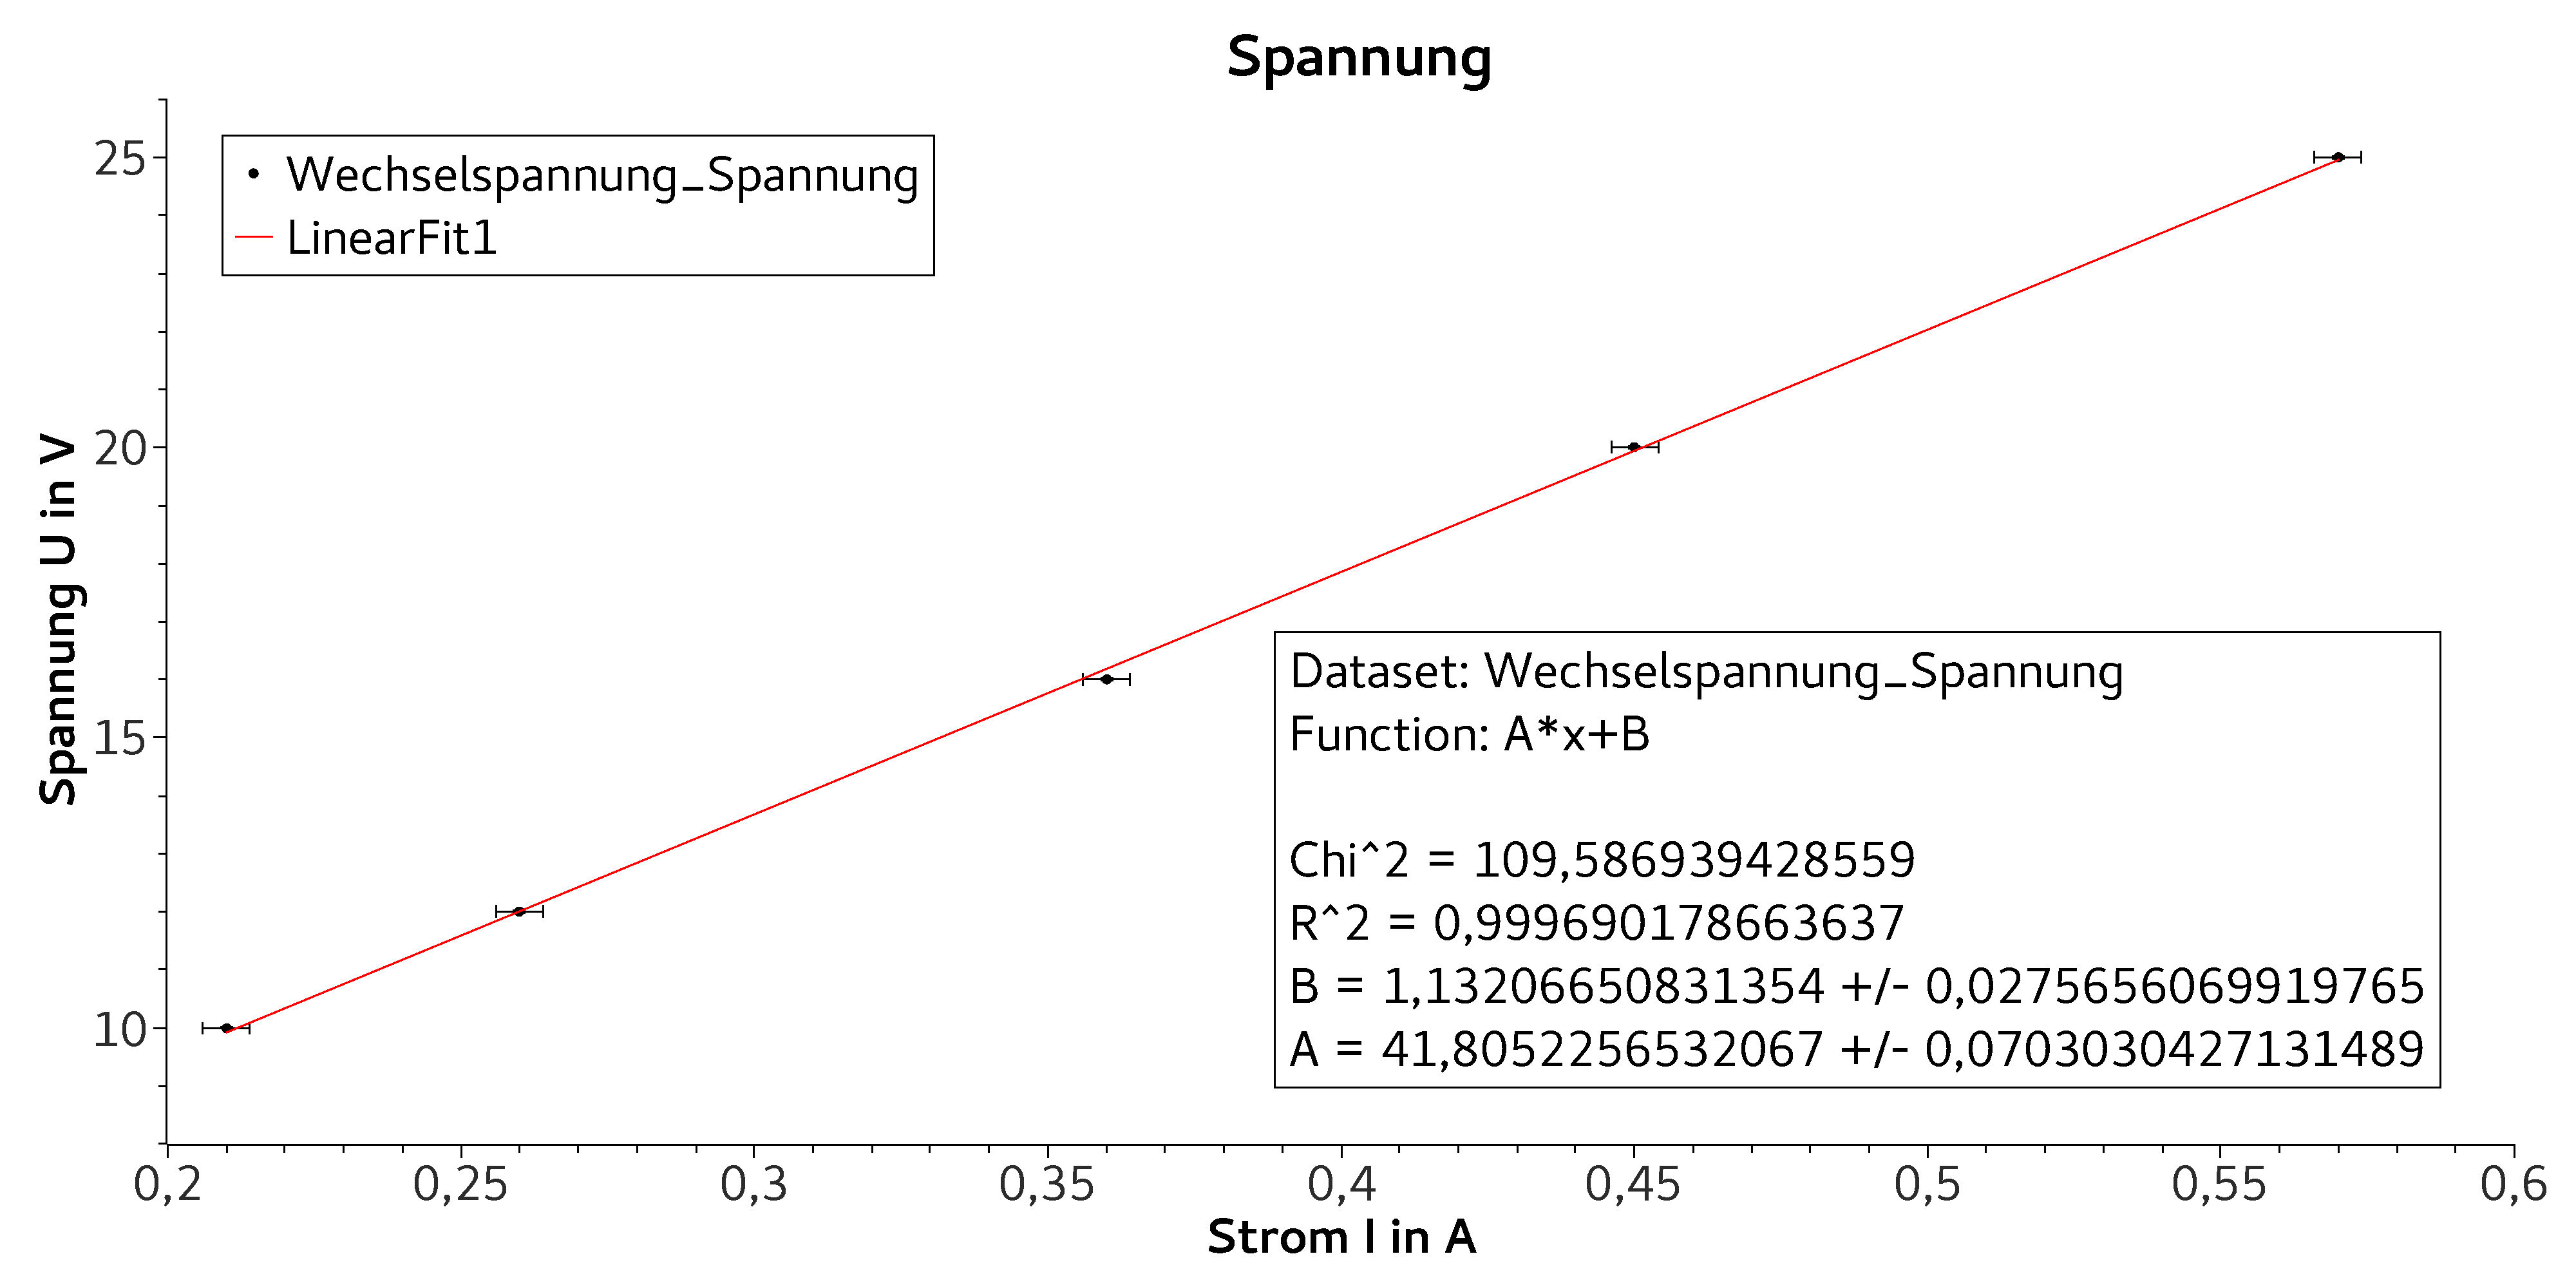
\includegraphics[width=1\textwidth]{KondensatorSpannungWechsel}
		\centering
		\caption{Die gemessene effektive Wechselspannung über eine Spule und einen Kondensator ist gegen den effektiven Wechselstrom aufgetragen.}
		\label{KondensatorSpannungWechsel}
		\centering
	\end{figure}
	\begin{figure}[tb]
		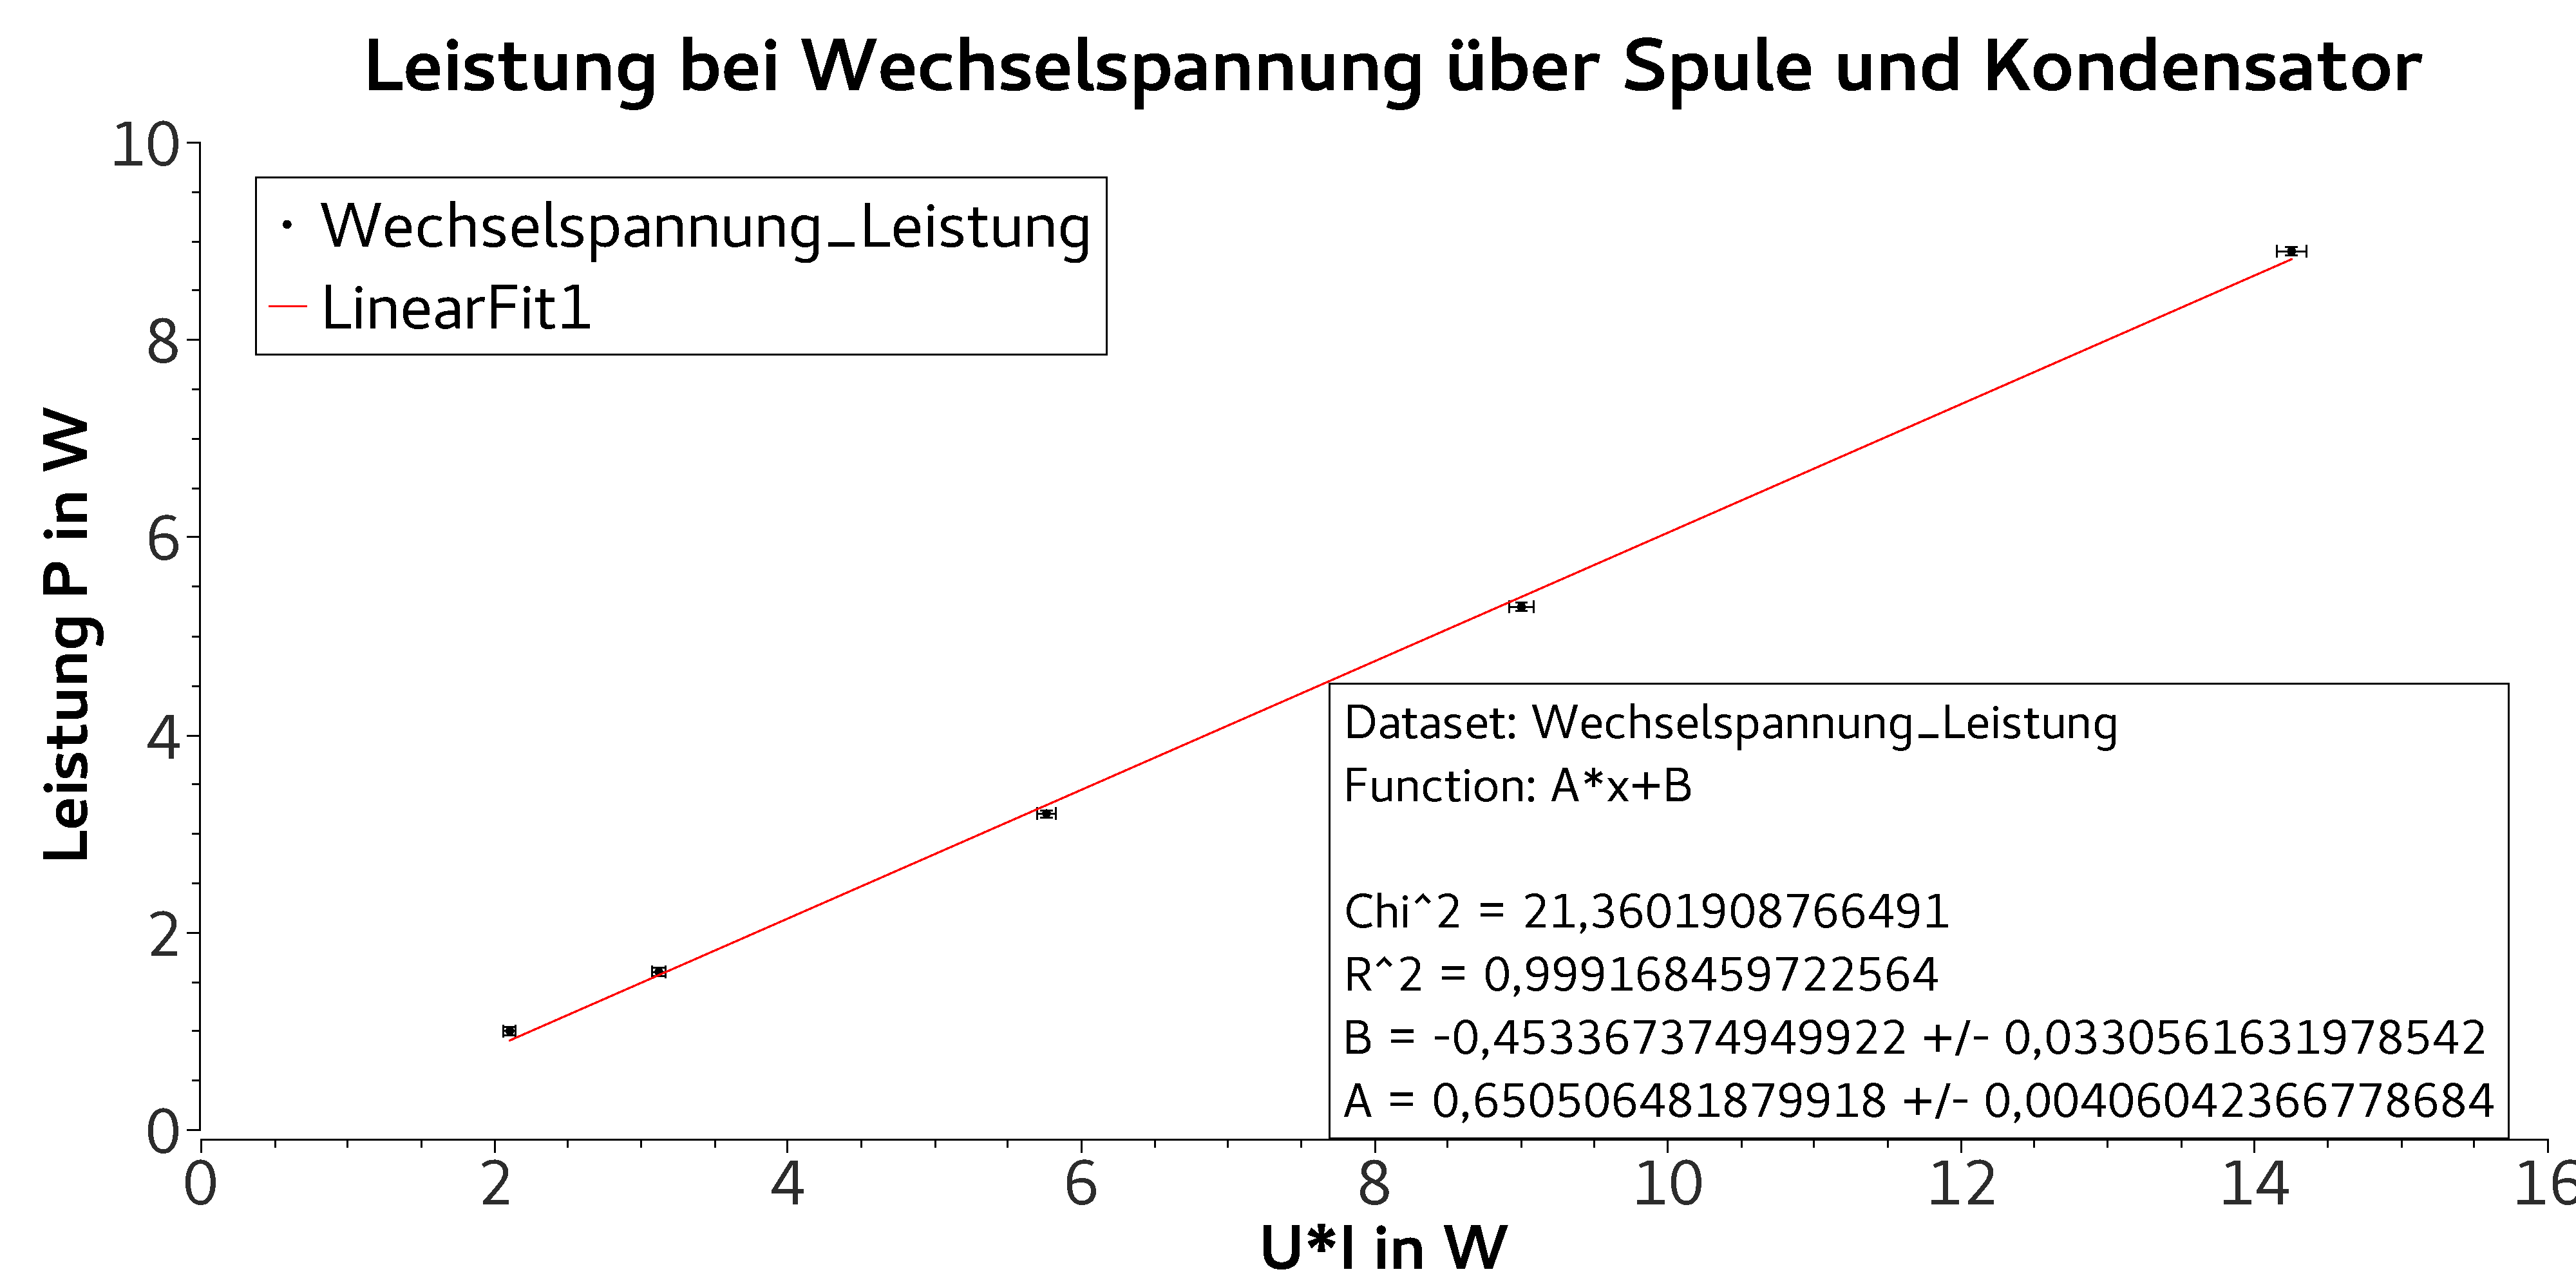
\includegraphics[width=1\textwidth]{KondensatorLeistungWechsel}
		\centering
		\caption{Die gemessene effektive Leistung ist gegen das Produkt aus Wechselstrom und Wechselspannung über eine Spule und einen Kondensator aufgetragen.}
		\label{KondensatorLeistungWechsel}
		\centering
	\end{figure}
	



	




	\subsection{Diskussion}
	%TODO Bezug/Nutzten oder sonst was
	%TODO auch hier die Hypothese wiederholen
	\subsubsection{Innenwiderstand}
	Erwartet war, dass der sich aus den Messungen ergebende Innenwiderstand sich nicht deutlich von dem zusätzlich angelöteten Widerstand unterscheidet.
	Tatsächlich wurde jedoch ein Wert von $R_\text{i} = \SI{29,51 \pm 0,59}{\Omega}$ gemessen.
	Dieser unterscheidet sich deutlich vom Wert von $R_\text{i} = \SI{18 \pm 0,18}{\Omega}$ , der vom angelöteten Widerstand abgelesen wurde.
	Dies kann entweder darauf zurückgeführt werden, dass der tatsächliche Innenwiderstand der Akkumulatoren deutlich höher als erwartet ist, dass der Widerstand vom angelöteten Widerstand falsch abgelesen wurde oder dass die Spannung vom Messgerät falsch abgelesen wurde.
	Es fällt weiterhin auf, dass sich für den Innenwiderstand der einzelnen Zellen ähnliche Werte (\cref{Tabelle_Innenwiderstaende2}) ergeben, was das Vorliegen eines der oberen Fälle unterstützt.
	
	\subsubsection{Gleich- und Wechselstrom mit verschiedenen Verbrauchern}
	
	Bei Verwendung eines einfachen Widerstandes war zu erwarten, dass der experimentell ermittelte Widerstand mit dem grob vom Potentiometer abgelesenen Widerstand innerhalb der Unsicherheitsintervalle übereinstimmen.
	Dies konnten die Messwerte von $R$ $\SI{15,72 \pm 0,04}{\Omega}$ bzw. $\SI{15,55 \pm 0,04}{\Omega}$ bei einem grob vom Potentiometer abgelesenen Wert von \SI{14 \pm 1,7}{\Omega} bestätigen.
	Das Auftragen der Leistung gegen das Produkt aus Strom und Spannung (vgl. \crefrange{WiderLeistungGleich}{WiderLeistungWechsel}) sollte eine Gerade der Steigung 1, die durch den Nullpunkt verläuft ergeben.
	Tatsächlich konnte jedoch wie in \cref{WiderLeistungGleich} und \cref{WiderLeistungWechsel} zusehen nur ein deutlich kleinerer Wert gemessen werden, der deutlich außerhalb der Unsicherheitsintervalle liegt.
	Im Fall von Wechselstrom könnte man hier eine Spuleneigenschaft des Potentiometers vermuten, da dieses den Widerstand über einen gewickelten Draht im Inneren realisierte, aber im Fall von Gleichstrom kann dies nicht Grund der Abweichung sein.
	Deshalb bleibt nur ein Messfehler beim Ablesen eines der Messgeräte als Erklärung übrig, wenn die Gültigkeit der Gleichung $ U \cdot I = P $ nicht infrage gestellt wird.
	\par
	Der Innen- und Wirkwiderstand und Phasenwinkel der Spule ist nur für die konkret verwendete Spule interessant und kann nicht mit einem Erwartungswert in Verbindung gebracht werden.
	Es lässt sich jedoch feststellen, dass der Wirkwiderstand $ R_W = \SI{23,9 \pm 0,06}{\ohm}$ sehr nah am Innenwiderstand der Spule von $ R_i = \SI{24,04}{\ohm} $.
	Dies ist war auch zu erwarten, da der Wirkwiderstand der Realteil, also der bei Gleichstrom gemessene Teil, des Scheinwiderstands ist.
	Die geringe Abweichung lässt sich durch ein Steigen des Widerstands der Spule bei Betrieb erklären, da die Erwärmung der Spule ein Steigen des Widerstandes zur Folge hat.
	\par 
	Bei Messung mit einem Verbraucher in Form von von Spule und Kondensator konnte Betrag und Phase des Wechselstromwiderstandes bestimmt werden.
	Auch die Kapazität des Kondensators wurde bestimmt und liegt mit \SI{63,8 \pm 2,1}{\micro \farad} nah an der auf dem Kondensator angegebenen Kapazität von \SI{60}{\micro \farad}, welche innerhalb der doppelten Unsicherheit liegt.
	Da die Angabe auf dem Kondensator keine Unsicherheit enthielt, lässt sich nicht eindeutig sagen, ob die Angabe des Herstellers bestätigt werden konnte.
	
	\section{Schlussfolgerung}
	%TODO Rückgriff auf Hypothese und drittes Nennen dieser
	Im Fall der Innenwiderstände von Akkumulatorzellen konnte der Innenwiderstand der Akkumulatorzellen nicht eindeutig bestimmt werden.
	Das Ergebnis eines deutlich höheren Innenwiderstandes als erwartet bedeutet, dass entweder ein Fehler in der Vorgehensweise beim Messen vorliegt oder die Hypothese, dass der eigentliche Innenwiderstand in der Dimension kleiner ist als der angelötete Widerstand, verworfen werden muss.
	Bei der Verlustleistung verschiedener Verbraucher konnte bei einem ohmschen Widerstand als Verbraucher der gemessene Wert des Widerstandes den grob abgeschätzten bestätigen.
	Nicht bestätigt werden konnte der Zusammenhang zwischen Strom, Spannung und Leistung.
	Bei einer Spule als Verbraucher wurde Wirkwiderstand, Phasenwinkel, Induktivität und Innenwiderstand bestimmt, aber diese Werte konnten anhand mangelnder Angaben auf der Spule leider nicht verglichen werden.
	Allerdings konnte hier die Vermutung bestätigt werden, dass der Realteil der Impedanz einer Spule dem Wirkwiderstand und somit dem bei Gleichstrombetrieb gemessenen Innenwiderstand entspricht.
	Wenn als Verbraucher Spule und Kondensator angeschlossen war, konnte die Vermutung, dass die gemessene Kapazität des Kondensators mit der auf ihm angegebenen übereinstimmt, innerhalb annehmbarer Wahrscheinlichkeiten bestätigt werden, aber um eine sinnvolle Überprüfbarkeit der Herstellerangaben zu erlauben, müsste dieser zusätzlich eine Unsicherheit der Kapazität auf dem Bauteil angegeben.
	
	%TODO Quellen zitieren, Websiten mit Zugriffsdatum
	%TODO Verweise auf das Laborbuch (sind erlaubt)
	%TODO Tabelle + Bilder mit Beschriftung
	%\printbibliography
\end{document}
